%% History:
% Pavel Tvrdik (26.12.2004)
%  + initial version for PhD Report
%
% Daniel Sykora (27.01.2005)
%
% Michal Valenta (3.12.2008)
% rada zmen ve formatovani (diky M. Duškovi, J. Holubovi a J. Žďárkovi)
% sjednoceni zdrojoveho kodu pro anglickou, ceskou, bakalarskou a diplomovou praci

% One-page layout: (proof-)reading on display
%%%% \documentclass[11pt,oneside,a4paper]{book}
% Two-page layout: final printing
\documentclass[11pt,twoside,a4paper]{book}   
%=-=-=-=-=-=-=-=-=-=-=-=--=%
% The user of this template may find useful to have an alternative to these 
% officially suggested packages:
\usepackage[czech, english]{babel}
\usepackage[T1]{fontenc} % pouzije EC fonty 
% pripadne pisete-li cesky, pak lze zkusit take:
% \usepackage[OT1]{fontenc} 
\usepackage[utf8]{inputenc}
%=-=-=-=-=-=-=-=-=-=-=-=--=%
% In case of problems with PDF fonts, one may try to uncomment this line:
%\usepackage{lmodern}
%=-=-=-=-=-=-=-=-=-=-=-=--=%
%=-=-=-=-=-=-=-=-=-=-=-=--=%
% Depending on your particular TeX distribution and version of conversion tools 
% (dvips/dvipdf/ps2pdf), some (advanced | desperate) users may prefer to use 
% different settings.
% Please uncomment the following style and use your CSLaTeX (cslatex/pdfcslatex) 
% to process your work. Note however, this file is in UTF-8 and a conversion to 
% your native encoding may be required. Some settings below depend on babel 
% macros and should also be modified. See \selectlanguage \iflanguage.
%\usepackage{czech}  %%%%%\usepackage[T1]{czech} %%%%[IL2] [T1] [OT1]
%=-=-=-=-=-=-=-=-=-=-=-=--=%

%%%%%%%%%%%%%%%%%%%%%%%%%%%%%%%%%%%%%%%
% Styles required in your work follow %
%%%%%%%%%%%%%%%%%%%%%%%%%%%%%%%%%%%%%%%
\usepackage{graphicx}
\usepackage{indentfirst} %1. odstavec jako v cestine.
\usepackage{k336_thesis_macros} % specialni makra pro formatovani DP a BP
 % muzete si vytvorit i sva vlastni v souboru k336_thesis_macros.sty
 % najdete  radu jednoduchych definic, ktere zde ani nejsou pouzity
 % napriklad: 
 % \newcommand{\bfig}{\begin{figure}\begin{center}}
 % \newcommand{\efig}{\end{center}\end{figure}}
 % umoznuje pouzit prikaz \bfig namisto \begin{figure}\begin{center} atd.


%%%%%%%%%%%%%%%%%%%%%%%%%%%%%%%%%%%%%
% Zvolte jednu z moznosti 
% Choose one of the following options
%%%%%%%%%%%%%%%%%%%%%%%%%%%%%%%%%%%%%
%\newcommand\TypeOfWork{Diplomová práce} \typeout{Diplomova prace}
% \newcommand\TypeOfWork{Master's Thesis}   \typeout{Master's Thesis} 
 \newcommand\TypeOfWork{Bakalářská práce}  \typeout{Bakalarska prace}
% \newcommand\TypeOfWork{Bachelor's Project}  \typeout{Bachelor's Project}


%%%%%%%%%%%%%%%%%%%%%%%%%%%%%%%%%%%%%
% Zvolte jednu z moznosti 
% Choose one of the following options
%%%%%%%%%%%%%%%%%%%%%%%%%%%%%%%%%%%%%
% nabidky jsou z: http://www.fel.cvut.cz/cz/education/bk/prehled.html

%\newcommand\StudProgram{Elektrotechnika a informatika, dobíhající, Bakalářský}
%\newcommand\StudProgram{Elektrotechnika a informatika, dobíhající, Magisterský}
% \newcommand\StudProgram{Elektrotechnika a informatika, strukturovaný, Bakalářský}
% \newcommand\StudProgram{Elektrotechnika a informatika, strukturovaný, Navazující magisterský}
 \newcommand\StudProgram{Softwarové technologie a management, Bakalářský}
% English study:
% \newcommand\StudProgram{Electrical Engineering and Information Technology}  % bachelor programe
% \newcommand\StudProgram{Electrical Engineering and Information Technology}  %master program


%%%%%%%%%%%%%%%%%%%%%%%%%%%%%%%%%%%%%
% Zvolte jednu z moznosti 
% Choose one of the following options
%%%%%%%%%%%%%%%%%%%%%%%%%%%%%%%%%%%%%
% nabidky jsou z: http://www.fel.cvut.cz/cz/education/bk/prehled.html

%\newcommand\StudBranch{Výpočetní technika}   % pro program EaI bak. (dobihajici i strukt.)
%\newcommand\StudBranch{Výpočetní technika}   % pro prgoram EaI mag. (dobihajici i strukt.)
\newcommand\StudBranch{Softwarové inženýrství}            %pro STM
%\newcommand\StudBranch{Web a multimedia}                  % pro STM
%\newcommand\StudBranch{Computer Engineering}              % bachelor programe
%\newcommand\StudBranch{Computer Science and Engineering}  % master programe


%%%%%%%%%%%%%%%%%%%%%%%%%%%%%%%%%%%%%%%%%%%%
% Vyplnte nazev prace, autora a vedouciho
% Set up Work Title, Author and Supervisor
%%%%%%%%%%%%%%%%%%%%%%%%%%%%%%%%%%%%%%%%%%%%

\newcommand\WorkTitle{Demonstrační aplikace pro podporu kurzu neuronových sítí}
\newcommand\FirstandFamilyName{Adam Činčura}
\newcommand\Supervisor{Ing. Zdeněk Buk}


% Pouzijete-li pdflatex, tak je prijemne, kdyz bude mit vase prace
% funkcni odkazy i v pdf formatu
\usepackage[
pdftitle={\WorkTitle},
pdfauthor={\FirstandFamilyName},
bookmarks=true,
colorlinks=true,
breaklinks=true,
urlcolor=red,
citecolor=blue,
linkcolor=blue,
unicode=true,
]
{hyperref}



% Extension posted by Petr Dlouhy in order for better sources reference (\cite{} command) especially in Czech.
% April 2010
% See comment over \thebibliography command for details.

\usepackage[square, numbers]{natbib}             % sazba pouzite literatury
%\usepackage{url}
%\DeclareUrlCommand\url{\def\UrlLeft{<}\def\UrlRight{>}\urlstyle{tt}}  %rm/sf/tt
%\renewcommand{\emph}[1]{\textsl{#1}}    % melo by byt kurziva nebo sklonene,
\let\oldUrl\url
\renewcommand\url[1]{<\texttt{\oldUrl{#1}}>}




\begin{document}

%%%%%%%%%%%%%%%%%%%%%%%%%%%%%%%%%%%%%
% Zvolte jednu z moznosti 
% Choose one of the following options
%%%%%%%%%%%%%%%%%%%%%%%%%%%%%%%%%%%%%
\selectlanguage{czech}
%\selectlanguage{english} 

% prikaz \typeout vypise vyse uvedena nastaveni v prikazovem okne
% pro pohodlne ladeni prace


\iflanguage{czech}{
	 \typeout{************************************************}
	 \typeout{Zvoleny jazyk: cestina}
	 \typeout{Typ prace: \TypeOfWork}
	 \typeout{Studijni program: \StudProgram}
	 \typeout{Obor: \StudBranch}
	 \typeout{Jmeno: \FirstandFamilyName}
	 \typeout{Nazev prace: \WorkTitle}
	 \typeout{Vedouci prace: \Supervisor}
	 \typeout{***************************************************}
	 \newcommand\Department{Katedra počítačů}
	 \newcommand\Faculty{Fakulta elektrotechnická}
	 \newcommand\University{České vysoké učení technické v Praze}
	 \newcommand\labelSupervisor{Vedoucí práce}
	 \newcommand\labelStudProgram{Studijní program}
	 \newcommand\labelStudBranch{Obor}
}{
	 \typeout{************************************************}
	 \typeout{Language: english}
	 \typeout{Type of Work: \TypeOfWork}
	 \typeout{Study Program: \StudProgram}
	 \typeout{Study Branch: \StudBranch}
	 \typeout{Author: \FirstandFamilyName}
	 \typeout{Title: \WorkTitle}
	 \typeout{Supervisor: \Supervisor}
	 \typeout{***************************************************}
	 \newcommand\Department{Department of Computer Science and Engineering}
	 \newcommand\Faculty{Faculty of Electrical Engineering}
	 \newcommand\University{Czech Technical University in Prague}
	 \newcommand\labelSupervisor{Supervisor}
	 \newcommand\labelStudProgram{Study Programme} 
	 \newcommand\labelStudBranch{Field of Study}
}




%%%%%%%%%%%%%%%%%%%%%%%%%%    Poznamky ke kompletaci prace
% Nasledujici pasaz uzavrenou v {} ve sve praci samozrejme 
% zakomentujte nebo odstrante. 
% Ve vysledne svazane praci bude nahrazena skutecnym 
% oficialnim zadanim vasi prace.
%{
%\pagenumbering{roman} \cleardoublepage \thispagestyle{empty}
%\chapter*{Na tomto místě bude oficiální zadání vaší práce}
%\begin{itemize}
%\item Toto zadání je podepsané děkanem a vedoucím katedry,
%\item musíte si ho vyzvednout na studiijním oddělení Katedry %počítačů na Karlově náměstí,
%\item v jedné odevzdané práci bude originál tohoto zadání (originál %zůstává po obhajobě na katedře),
%\item ve druhé bude na stejném místě neověřená kopie tohoto %dokumentu (tato se vám vrátí po obhajobě).
%\end{itemize}
%\newpage
%}

%%%%%%%%%%%%%%%%%%%%%%%%%%    Titulni stranka / Title page 

\coverpagestarts

%%%%%%%%%%%%%%%%%%%%%%%%%%%    Podekovani / Acknowledgements 

\acknowledgements
\noindent
Děkuji Ing. Zdeňku Bukovi za užitečné rady a připomínky k tvorbě této bakalářské práci.


%%%%%%%%%%%%%%%%%%%%%%%%%%%   Prohlaseni / Declaration 

\declaration{V~Praze dne 24.\,5.\,2011}
%\declaration{In Kořenovice nad Bečvárkou on May 15, 2008}


%%%%%%%%%%%%%%%%%%%%%%%%%%%%    Abstract 
 
\abstractpage

Demonstrational application created in this bachelor thesis is supposed to complete electronic attachment of lecture notes for the "Neural networks and neurocomputers" course. Application is created in Mathematica program with use of NeuralNetworks library. Every file allows to experiment with specific neural network or its parameteres. All experiments have enclosed explaining commentary. Final application was created by extension and completion of current demonstrational application.
% Prace v cestine musi krome abstraktu v anglictine obsahovat i
% abstrakt v cestine.
\vglue60mm

\noindent{\Huge \textbf{Abstrakt}}
\vskip 2.75\baselineskip

\noindent
Demonstrační aplikace vytvořená v rámci této bakalářské práce doplňuje elektronickou přílohu skript pro předmět \uv{Neuronové sítě a neuropočítače}. Aplikace je vytvořena v programu Mathematica s použitím knihovny NeuralNetworks. Každý soubor umožňuje snadno experimentovat s danou neuronovou sítí nebo s jejími parametry. Všechny experimenty jsou doprovázeny vysvětlujícím komentářem. Výsledná aplikace vznikla rozšířením a doplněním stávající demonstrační aplikace.

%%%%%%%%%%%%%%%%%%%%%%%%%%%%%%%%  Obsah / Table of Contents 

\tableofcontents


%%%%%%%%%%%%%%%%%%%%%%%%%%%%%%%  Seznam obrazku / List of Figures 

\listoffigures


%%%%%%%%%%%%%%%%%%%%%%%%%%%%%%%  Seznam tabulek / List of Tables

\listoftables


%**************************************************************

\mainbodystarts
% horizontalní mezera mezi dvema odstavci
%\parskip=5pt
%11.12.2008 parskip + tolerance
\normalfont
\parskip=0.2\baselineskip plus 0.2\baselineskip minus 0.1\baselineskip

% Odsazeni prvniho radku odstavce resi class book (neaplikuje se na prvni 
% odstavce kapitol, sekci, podsekci atd.) Viz usepackage{indentfirst}.
% Chcete-li selektivne zamezit odsazeni 1. radku nektereho odstavce,
% pouzijte prikaz \noindent.

%**************************************************************

% Pro snadnejsi praci s vetsimi texty je rozumne tyto rozdelit
% do samostatnych souboru nejlepe dle kapitol a tyto potom vkladat
% pomoci prikazu \include{jmeno_souboru.tex} nebo \include{jmeno_souboru}.
% Napr.:
% \include{1_uvod}
% \include{2_teorie}
% atd...

%*****************************************************************************
\chapter{Úvod}
Problematika neuronových sítí není triviální záležitostí. Pro pochopení principu fungování libovolné neuronové sítě je potřeba porozumět teoretickému fungování sítě. Tohoto porozumění se dosáhne snáze, pokud má student možnost si danou síť vlastnoručně osahat, nastavovat si její parametry, pozorovat výstupy a předkládat síti vlastní data. Z těchto důvodů má předmět \uv{Neuronové sítě a neuropočítače}, v rámci kterého je na FEL ČVUT problematika neuronových sítí vyučována, rozsáhlou elektronickou přílohu skript tzv. Courseware\cite{courseware}.

Součástí Courseware je také demonstrační aplikace v programu Mathematica, kterou jsem v rámci této bakalářské práce přepracoval a rozšířil. Demonstrační aplikace nevyžaduje téměř žádné znalosti programování v systému Mathematica, umožňuje velmi snadno měnit parametry a strukturu zadaných sítí, vizualizovat průběh učení sítě, vizualizovat výstup sítě a upravovat vstupní data. Celá aplikace je doplněna vysvětlujícím komentářem. Věřím, že moje práce pomůže studentům snáze se v neuronových sítích zorientovat.
\section{Vymezení cíle práce}
Cílem práce je provést úpravy a rozšíření stávající demonstrační aplikace. Výstup této práce nahradí stávající aplikaci a bude používán při výuce předmětu \uv{Neuronové sítě a neuropočítače}.
\section{Struktura práce}
 TODO až bude hotovo

%*****************************************************************************
\chapter{Umělé neuronové sítě}
\section{Historie}
Za počátek vzniku oboru neuronových sítí je považována práce Warrena McCullocha a Waltera Pittse z roku 1943, ve které vytvořili první, velmi jednoduchý model neuronu. V roce 1949 navrhl Donald Hebb učící pravidlo pro neuronové sítě. V roce 1957 vynalezl Frank Rosenblatt tzv. \textit{perceptron}, pro který navrhl také učící algoritmus. Krátce po objevu perceptronu vyvinul Bernard Widrow další typ neuronu ADALINE (ADAptive LINear Element). V této dochází ke značnému rozvoji neuronových sítí, neuronové sítě se začínají vyrábět jako hardwarové prvky. Přesto došlo koncem šedesátých let k výraznému útlumu výzkumu neuronových sítí. Důvodem toho byly nadměrné očekávání jako například vyvinutí umělého mozku. K opouštění výzkumu neuronových sítí vedla také kampaň Marvina Minského a Seymoura Papertema, kteří poukazovali na fakt, že jeden perceptron není schopen rozhodnout jednoduchou logickou úlohu tzv. XOR problém (vylučovací disjunkce). Z toho vyvodili, že výzkum neuronových sítí není perspektivní.

Další výzkum neuronových sítí nastartovala na počátku osmdesátých let americká grantová agentura DARPA (Defense Advanced Reseach Project Agency), který začala výzkum neuronových sítí finančně podporovat. Výsledky se dostavily v podobě objevu algoritmu zpětné propagace chyby (backpropagation) a vynálezu Hopieldovy neuronové sítě. Tyto objevy obnovily zájem veřejnosti i vědců o neuronové sítě. Objev SOM (Self Organizing Map) Teuva Kohonena přinesl novou myšlenku do oblasti neuronových sítí a to učení sítě bez učitele. Další výzkum neuronových sítí probíhá dodnes. Podrobnější historii je možné nalézt v\cite{teoret}.

\section{Aplikace}

\begin{itemize}
\item Klasifikace

Klasifikace, někdy také označována jako rozpoznávání, je jedna z nejjednodušších aplikací neuronových sítí. Úkolem klasifikace je rozhodnout do které ze tříd (kategorií) vstupní vektor patří.
\newpage
\item Predikce

Predikcí se rozumí předpovídání výstupní hodnoty na základě znalosti jejího průběhu v minulosti. Výhoda neuronových sítí pro predikci spočívá v automatickém naučení pouze z naměřených hodnot, bez nutnosti dodávat další informace a také vysoká schopnost adaptace. Neuronové sítě dokáží odhalit i silně nelineární závislosti. Nevýhodou může být, že se neuronová síť naučí závislost, která je platná pouze v omezeném úseku dat. 
\item Aproximace

Aproximace spočívá v přibližném určení hodnoty. Aproximace může například sloužit k určení průběhu funkce na základě navzorkovaných hodnot této funkce. Je výhodné ji použít pokud by výpočet této hodnoty nebyl možný případně velmi neefektivní.
\item Shluková analýza

Cílem shlukové analýzy je nalézt v množině objektů (dat) takové její podmnožiny (shluky), aby si objekty v každém shluku byly vzájemně podobné a zároveň si nebyly příliš podobné s objekty mimo daný shluk. Ke shlukové analýze dat je možné s výhodou použít sítě, které používají učení bez učitele např. samoorganizující se mapy.
\item Filtrace slouží

Filtrace slouží k vyhlazení průběhu signálu, případně k odstranění šumu. Na vstup neuronové sítě se přivede šumem poškozený signál a z výstupu neuronové sítě je získán nezkreslený výstupní signál. Velmi podobnou funkci jako filtrace umožňuje asociace. Na rozdíl od filtrace je při asociaci neuronová síť naučena na datech bez šumu a poté zpracovává zašuměná data.
\item Komprese dat

Komprese dat pomocí neuronové sítě je vhodná především pro kompresi videa například při videokonferencích nebo u televizního vysílání. Ke kompresi jdou nejlépe využít vícevrstvé perceptronové sítě.
\end{itemize}

\section{Využití}
Neuronové sítě se používají všude tam, kde nám nevadí případná chyba (neuronové sítě dosahují úspěšnosti okolo 95\%) a kde je přesný algoritmus náročný na finanční prostředky (hardware) nebo na čas (potřeba rychle rozhodnout). Dále je možné neuronové sítě použít k řešení problému, k jejichž řešení neznáme přesný algoritmus. Následuje několik konkrétních příkladů použití neuronových sítí.

Neuronové sítě byly využity v systému AMT, který optimalizuje rezervace letenek. V první fázi neuronová síť předpovídá poptávku po volných místech v letadlech. Podle těchto předpovědí se navrhuje rozložení letů.

Neuronové sítě jsou používány také ve zdravotnictví k analýze EKG křivky, ve které vyhledává určité složky, čímž dokáže ušetřit velké množství času lékařům, kteří by záznam procházeli ručně. Existuje také systém, který na základě analýzy EKG křivky umožňuje odhadnout nemoc pacienta. Další využití v lékařství je při podávání antibiotik, kdy neuronová síť pracovala 4\begin{math}\times\end{math} přesněji než lékaři (např. nepředepisovala antibiotika, na které mohl být pacient alergický). Lékařům sloužila jako konzultant.

Další poměrně lákavé využití přináší finančnictví. Pomocí neuronových sítí se predikuje vývoj kurzů měn a také vývoj kurzu akcií. Zatímco při použití klasických metod je úspěšnost predikce cca 55\%, při použití neuronových sítí se dosahuje až 75\%. Stejným způsobem se pomocí neuronových sítí predikuje spojení a krach podniků. Jiným využitím ve finančnictví je testování, zda daný klient bude schopen splácet půjčku, případně navrhnutí výše půjčky a doby splácení.

Neuronovou síť je možné použít k řízení výrobní linky, případně celého závodu. Nejprve je neuronová síť nainstalována a učí se reagovat na podněty od svého \uv{učitele} - člověka vykonávajícího stejnou práci, která se požaduje od neuronové sítě. Poté, co je síť dostatečně naučena je schopna reagovat správně i na neznáme podněty. Podobným způsobem byly provedeny pokusy, při kterých se neuronová síť učila řídit automobil. Naučená síť potom řídila podobným způsobem jako její \uv{učitel} - agresivně brzda, plyn, nebo naopak opatrně.\cite{kacenka}

%*****************************************************************************
\chapter{Umělý neuron}
\section{Biologický předobraz umělého neuronu}
Umělé neuronové sítě vznikly na základě svého biologického předobrazu - nervové soustavy. Nervová soustava se skládá s mnoha vzájemně propojených výkonných buněk - neuronů. Neurony mají za úkol zpracování, přenos a uchování informace. Každý neuron je vzájemně propojen se stovkami jiných neuronů, kterých se v lidském těle nachází přibližně 10\begin{math} ^{12}\end{math}.\cite{skripta}

Základem biologického neuronu je buněčné tělo s jádrem (soma), z něj vychází jediný rozvětvený výstup zvaný axon. Axon je zakončen takzvanými terminály axonu, ty se dotýkají dendritů ostatních neuronů a slouží k předávání vzruchů ostatním neuronům. Dendrity slouží naopak k přijímání vzruchů od ostatních neuronů. Strukturu biologického neuronu si můžete prohlédnout na obrázku~\ref{fig:bioneuron} Vlastní přenos vzruchů, tedy informací, zprostředkovávají chemické synapse. Tyto synapse mohou vzruch utlumit nebo zesílit. Učení biologické neuronové sítě je založeno na změně reakce synapse na daný vzruch, případně vytvoření nové synapse nebo zánik stávající.

\begin{figure}[!h]
\begin{center}
\includegraphics[height=6cm]{figures/bioneuron.png}
\caption{Biologický neuron\cite{teoret}}
\label{fig:bioneuron}
\end{center}
\end{figure}

\section{Struktura umělého neuronu}
Základním stavebním kamenem neuronových sítí je model neuronu. Nejrozšířenějším modelem neuronu je McCulloch-Pittsův perceptron, pojmenovaný dle svých vynálezců.  Model tohoto neuronu vidíte na obrázku~\ref{fig:perceptron}. Neuron má konečný počet vstupů \begin{math} x_{1}\end{math} až \begin{math}x_{n}\end{math}, každý vstup \begin{math} x_{i}\end{math} je ohodnocen vahou \begin{math} w_{i}\end{math}. Dále je každý neuron vybaven aktivační funkcí \begin{math}S\end{math}, prahovou hodnotou \begin{math}\theta\end{math} a jedním výstupem \begin{math} y\end{math}. Výstup neuronu se řídí následující rovnicí.
\begin{equation}
  y=S(\sum\limits_{i=1}^N w_{i}x_{i} + \theta)
\end{equation}

\begin{figure}[!h]
\begin{center}
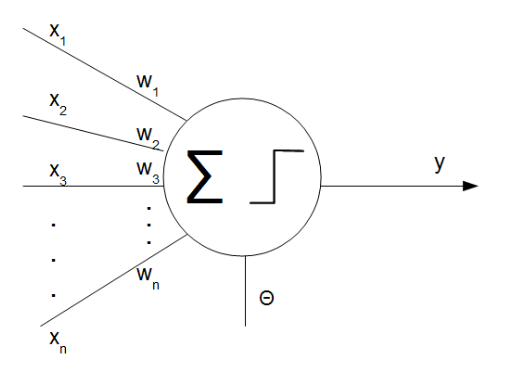
\includegraphics[height=6cm]{figures/perceptron.png}
\caption{McCulloch-Pittsův perceptron}
\label{fig:perceptron}
\end{center}
\end{figure}

Na vstupy neuronu se přivádí data ze vstupní množiny (mohou být reálná i binární), nebo spojitá data. Každý vstup \begin{math} x_{i}\end{math} je modifikován vahou daného vstupu \begin{math} w_{i}\end{math}. Tyto váhy vstupů se během učení mění, což představuje základ učení neuronu. Významným vstupům, které výrazně ovlivňují výstup neuronu se přiřazuje vyšší váha a naopak méně významným vstupům se váha snižuje.

Práh je hodnota, po jejímž překročení se neuron stává aktivním. Hodnota prahu se spočítá jako vážený součet vstupů. Pokud tento součet nepřekročí prahovou hodnotu, zůstává neuron neaktivní. Práh je často realizován jako další vstup neuronu s konstantní hodnotou \begin{math} x_{0}=1\end{math}, váha \begin{math} w_{0}\end{math} potom označuje samotný práh. Funkce pro výpočet výstupu poté vypadá následovně.

\begin{equation}
  y=S(\sum\limits_{i=0}^N w_{i}x_{i} + \theta),\; kde\; x_{0}=1
\end{equation}

Přenosová funkce je funkce, pomocí které je transformován vnitřní potenciál neuronu do požadovaného oboru hodnot. Pomocí vhodné volby přenosové funkce může neuron produkovat binární nebo spojitý výstup. Pro binární výstup se používají skoková a Heavisideova funkce, pro spojitý výstup se používají saturovaná lineární funkce, Gaussovská funkce, sigmoidní funkce a hyperbolický tangens.\citep{teoret}

\section{Proces učení}
Při učení dochází v neuronové síti ke změnám, kterými se síť adaptuje na řešení daného problému. Učení je u umělé neuronové sítě realizováno nastavováním vah a prahů jednotlivých neuronů. Během učení nedochází nikdy ke změně struktury sítě (s výjimkou sítě GMDH, která není v tomto textu rozebírána). Před začátkem učení se obvykle nastaví váhy a prahy neuronů na náhodné hodnoty.

U učení umělé neuronové sítě můžeme pozorovat paralelu s učením biologické neuronové sítě, kdy v obou případech dochází k opakovanému předkládání vstupních dat a kontrole výstupu. Tímto opakováním se obě sítě učí dokud nereagují na předávané vstupy správně, nebo jen s akceptovatelnou odchylkou, tedy dokud nejsou naučeny.

Existují dva způsoby učení neuronové sítě:
\begin{itemize}
\item Učení s učitelem

Při učení s učitelem máme k dispozici trénovací množinu, která se skládá ze vstupních vektorů a jim odpovídajícím výstupních vektorů. Učení probíhá postupným předkládáním trénovacích vzorů. Ke každému vzoru ve vypočte odchylka od požadovaného výstupu a na základě této odchylky se upravují hodnoty vah. Váhy se upraví tak, aby při opětovném předložení vzoru byla odchylka od požadovaného výstupu menší. Tato úprava se řídí učicím algoritmem (probrán dále). Změna vah při jednom učicím kroku je obvykle malá. Poté se předloží nový vzor a celý proces se opakuje. Učicí vzory jsou síti předkládány opakovaně a po provedení dostatečného počtu opakování začne síť podávat stabilní výstup v reakci na předkládaný vstup.

\item Učení bez učitele

Při učení bez učitele nemá neuronová síť žádné vnější kritérium správnosti, má k dispozici pouze vstupní vektory. Síť tedy operuje pouze s informacemi, které získala během učení. Algoritmus učení bez učitele je navržen tak, aby hledal ve vstupních datech vzorky se společnými vlastnostmi. Učení bez učitele je také nazýváno samoorganizací.
\end{itemize}
Existuje také učení jednorázové, kdy je síti předložen vzor a síť si jej zapamatuje. Takováto schopnost učení je u neuronových sítí poměrně neobvyklá. Jednorázového učení je schopna například Hopfieldova síť.
\section{Proces vybavování}
Vybavování je aktivní fází neuronové sítě a zpracovávají se v ní vstupní data. Neuronová síť, stejně jako lidská mysl, pracuje asociativním způsobem.\citep{skripta} Asociativní paměť pracuje na principu asociovaných prvků např. obličej a jméno člověka, kdy si po spatření člověka vybavíme jeho jméno.

Vybavování je možné rozlišit do dvou variant:
\begin{itemize}
\item Autoasociativní vybavování

Při autoasociativním vybavování dochází k vybavování stejného vektoru, který je předložen. Toto se může zdát nepraktické. Tuto vlastnost ale oceníme pokud je náš vzor poškozený nebo neúplný a neuronová síť nám ho dovede opravit. K tomuto účelu se také autoasociativní vybavování používá.
\item Heteroasociativní vybavování

Při heteroasociativním vybavování dochází po předložení vzoru k vybavení jiného vzoru, který je předloženým asociován. Typickým použitím této varianty vybavování je klasifikace vektorů do tříd.
\end{itemize}

\section{Učicí algoritmy}
Nyní již víme že neuronová síť se učí pomocí změn vah vstupů u jednotlivých neuronů. Abychom mohli pozorovat a měřit rozdíly v úspěšnosti sítě v průběhu učení, je potřeba zavést nějakou metriku, pomocí které budeme úspěšnost sítě měřit. V praxi se jako metrika používá střední kvadratická chyba (anglicky Mean Squared Error, odtud skratka MSE). MSE sítě se spočítá pomocí následující rovnice, kde \begin{math}n\end{math} je počet vektorů v trénovací množině,  \begin{math}y_{i}\end{math} je výstup sítě po přivedení \textit{i}-tého prvku testovací množiny na vstup a \begin{math}o_{i}\end{math} je požadovaný výstup po přivedení \textit{i}-tého prvku z testovací množiny.
\begin{equation}
	MSE=\frac{1}{n}\sum\limits_{i=1}^n (y_{i}-o_{i})^{2} 
\end{equation}
Ještě výhodnější metrikou pro měření úspěšnosti sítě během trénování je RMSE (Root Mean Squared Error). Její největší předností je možnost přímo ji porovnat s výstupem sítě, protože je ve stejných jednotkách jako výstup. Hodnota RMSE se spočte následovně:
\begin{equation}
RMSE=\sqrt{MSE}
\end{equation}
Platí, že čím nižší hodnota RMSE, tím lépe je neuronová síť naučena. Učicí algoritmy se v průběhu učení snaží minimalizovat hodnotu RMSE, rozdíl mezi jednotlivými algoritmy tedy spočívá v postupu, jakým je tato hodnota minimalizována. Všechny popisované algoritmy pracují iterativně.
\subsection{Algoritmus nejvyššího poklesu}
Algoritmus začíná s náhodně inicializovaným vektorem vah neuronů a vyžaduje zadat výchozí velikost učicího kroku. V každé iteraci je vektor vah neuronů upraven tak, aby se posunul ve směru nejvyššího poklesu funkce MSE o velikost učicího kroku, pokud by toto posunutí nesnížilo hodnotu MSE, je velikost učicího kroku snížena na polovinu. Snižobvání probíhá dokud posunutí váhového vektoru nezpůsobí pokles hodnoty funkce MSE.  Na závěr iterace je velikost učicího kroku zdvojnásobena, čímž je získána předběžná velikost kroku pro příští iteraci. Algoritmus končí pokud dosáhne minima funkce MSE (může být lokální) nebo vyčerpá přidělený počet iterací.

Algoritmus nejvyššího poklesu je nejjednodušší algoritmus ze zde popisovaných. Potřebuje nejméně výpočetního výkonu a dosahuje mnohem horších výsledků než ostatní popisované algoritmy.\cite{nndocumentation}
\subsection{Gauss-Newton algoritmus}
Algoritmus začíná s náhodně inicializovaným vektorem vah. Na začátku každé iterace je nastavena velikost učicího kroku na hodnotu 1. Pro určení směru posunu je použita Gauss-Newtonova metoda, která pro výpočet využívá první a druhé derivace. Ve vypočteném směru je vektor vah posunut o velikost učicího kroku. Posun je uskutečněn pouze pokud způsobí pokles hodnoty funkce MSE, jinak je velikost kroku snížena o polovinu. Poté algoritmus pokračuje další iterací. Algoritmus končí pokud dosáhne minima funkce MSE (může být lokální) nebo vyčerpá přidělený počet iterací.

Gauss-Newton algoritmus je rychlý a spolehlivý algoritmus, který je využívaný v mnoha oblastech k řešení problémů s minimalizací funkcí. Pro řešení problémů v oblasti neuronových sítí nemusí být vždy nejvhodnější volbou, protože může docházet k výpočtům s hodnotami s velkým číselným rozsahem. Pokud k tomuto dojde, bude algoritmus konvergovat velmi pomalu a bude zdržovat celý učicí proces. \cite{nndocumentation}
\subsection{Levenberg-Marquardt algoritmus}
Algoritmus začíná, stejně jako předchozí algoritmy, s náhodně inicializovaným vektorem vah. Levenberg-Marquardt algoritmus představuje kompromis mezi dvěma předchozími algoritmy. Výsledný směr posunutí vektoru vah je zjednodušeně dán kompromisem mezi směry, které navrhují algoritmus nejvyššího poklesu a Gauss-Newton algoritmus.  Namísto velikosti učicího kroku, která je u tohoto algoritmu stále 1, se mění hodnota \begin{math}\lambda\end{math}. Na začátku každé iterace se algoritmus pokusí snížit hodnotu \begin{math}\lambda\end{math}, pokud by takováto snížená hodnota \begin{math}\lambda\end{math} nezaručila pokles MSE, je \begin{math}\lambda\end{math} naopak zvětšována dokud nedojde k žádanému poklesu. Hodnota \begin{math}\lambda\end{math} určuje, kterému z navrhovaných směrů bude algoritmus přikládat vyšší váhu. Pokud se \begin{math}\lambda\end{math} blíží k nule, chová se algoritmus jako Gauss-Newton algoritmus, pokud \begin{math}\lambda\end{math} dosahuje vysokých hodnot, chová se jako algoritmus nejvyššího poklesu. Algoritmus končí za stejných podmínek jako Gauss-Newton algoritmus.\cite{nndocumentation}\cite{learningmachines} 

Levenberg-Marquardt algoritmus představuje pravděpodobně nejlepší volbu trénovacího algoritmu pro neuronové sítě.

\subsection{Algoritmus zpětné propagace}
Algoritmus zpětné propagace začíná stejně jako ostatní algoritmy s náhodně inicializovaným vektorem vah. Před začátkem běhu je algoritmu třeba nastavit délku učicího kroku a momentum. Algoritmus zpětné propagace se chová velmi podobně jako algoritmus nejvyššího poklesu. Také sleduje směr nejvyššího poklesu funkce MSE, ale liší se v délce učicího kroku, která zůstává po celý běh algoritmu stejná. Momentum slouží jako jakási setrvačnost, která ovlivňuje směr posunu vektoru vah. Díky momentu dokáže algoritmus opustit některá lokální minima. 

Algoritmus zpětné propagace je jedním z nejstarších algoritmů pro učení neuronových sítí. I přes použití momenta, které umožní uniknutí z lokálního minima, se nedoporučuje algoritmu zpětné propagace používat. Namísto zpětné propagace se doporučuje použít některý z moderních učicích algoritmů a opakovat trénink pro několik různých, náhodně inicializovaných vektorů vah.\cite{nndocumentation}
%*****************************************************************************
\chapter{Neuronové sítě}
\section{Dopředná síť}
\section{RBF síť}
\section{Samoorganizující mapy}
\section{Hopfieldova síť}
\section{LVQ}
%*****************************************************************************
\chapter{Učení sítě}
\section{Rozdělení vstupních dat}
\section{Křížová validace}

%*****************************************************************************
\chapter{Implementační prostředí}
\section{Wolfram Mathematica}
Systém Mathematica od firmy Wolfram Research je sofistikovaný matematický nástroj, který umožňuje provádět numerické i symbolické výpočty. Systém obsahuje velké množství vestavěných funkcí a umožňuje i přidání dalších uživatelsky definovaných funkcí. Dále nabízí široké možnosti vizualizace dat ve 2D i 3D grafech. Neméně podstatnou funkcí je možnost exportu vyhodnoceného notebooku do formátu pdf. Díky tomu může demonstrační aplikaci vytvořenou v systému Mathematica, byť v omezené míře, využít i student, který nemá na svém počítači systém Mathematica nainstalovaný. Systém je možné rozšířit celou řadou knihoven, jednou z nich je i knihovna Neural Networks, kterou jsem využil ve své demonstrační aplikaci. Demonstrační aplikaci jsem programoval ve verzi Mathematica 8.0. Pro studium programování v Mathematice jsem použil knihy\cite{mathD} a \cite{mathP}.

\begin{figure}[!h]
\begin{center}
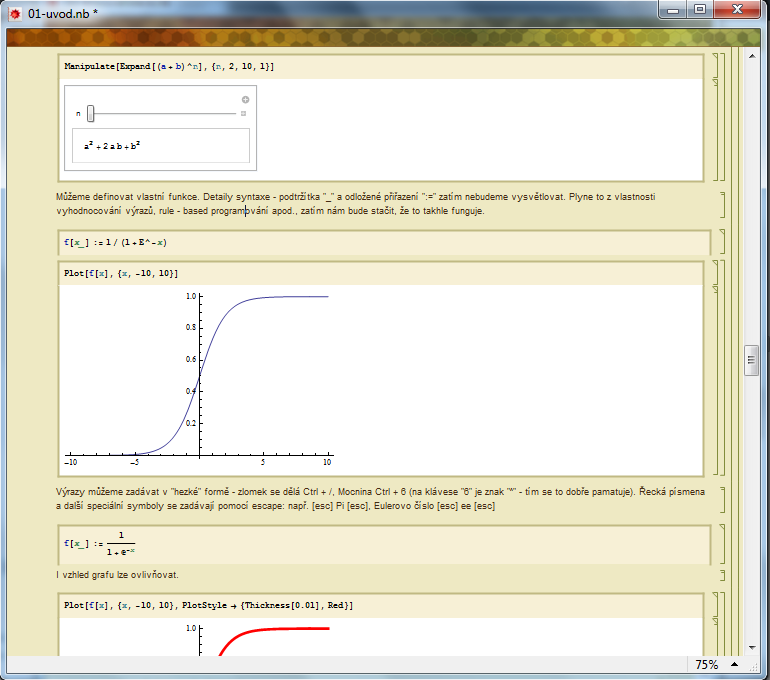
\includegraphics[height=10cm]{figures/ukazka01.png}
\caption{Ukázka prostředí systému Mathematica}
\label{fig:prostredi}
\end{center}
\end{figure}

\section{Knihovna Neural Networks}
Knihovna Neural Networks rozšiřuje systém \textit{Mathematica} o možnost pracovat s neuronovými sítěmi bez nutnosti vytvářet si její vlastní implementaci. Konkrétně knihovna nabízí práci s těmito konkrétními sítěmi: jednoduchý perceptron, dopředná neuronová síť, RBF neuronová síť, Hopfieldova neuronová síť, dynamická neuronová síť, Kohonenova mapa, LVQ a VQ. Knihovna také poskytuje implementaci různých algoritmů učení sítě, konkrétně jsou to tyto algoritmy: Levenberg-Marquardt, Gauss-Newton, gradientní algoritmus a algoritmus zpětné propagace. Knihovna umožňuje široké možnosti natavení parametrů u jednotlivých sítí a pro méně zkušené uživatele nabízí vytvoření sítě s výchozími parametry. Výchozí parametry jsou voleny tak, aby síť s výchozími parametry podávala dobré výkony a její učení a vybavování netrvalo přehnaně dlouho. Knihovna ještě nabízí široké možnosti vizualizace dat, grafické zobrazení průběhu učení sítě a také grafické zobrazení výstupu naučené neuronové sítě. Ke knihovně patří návod k použití a rozsáhlá dokumentace.
%*****************************************************************************
\chapter{Experimenty s neuronovými sítěmi}


\begin{center}
\begin{table}[h]
\begin{tabular}{|c|l|l|}
\hline 
Číslo kapitoly & Název kapitoly & Soubor \\ \hline
1 & Úvod & 01-uvod.nb \\ \hline
2 & Algoritmy učení & 02-algoritmy-uceni.nb \\ \hline
3 & Křížová validace & 03-krossvalidace.nb \\ \hline
4 & Dopředná síť a umělá data sin(x) & 04-feedforward-sin.nb \\ \hline
5 & Dopředná síť a Iris data & 05-feedforward-iris.nb \\ \hline
6 & Přístupy k učení dopředné sítě & 06-feedforward-iris-2.nb \\ \hline
7 & Pokrytí dat jednoduchou RBF sítí & 07-rbf-neuron.nb \\ \hline
8 & Pokrytí dat RBF sítí & 08-rbf-neuron-2.nb \\ \hline
9 & Síť RBF a umělá data sin(x) & 09-rbf-sin.nb \\ \hline
10 & Síť RBF  Iris data & 10-rbf-iris.nb \\ \hline
11 & Přístupy k učení RBF sítě & 11-rbf-iris-2.nb \\ \hline
12 & Hopfieldova síť a umělé vzory & 12-hopfield.nb \\ \hline
13 & Shlukování dat sítí bez učitele & 13-som-clustering.nb \\ \hline
14 & Kohonenova síť a Iris data & 14-som-iris.nb \\ \hline
15 & LVQ a Iris data & 15-lvq-iris.nb \\ \hline
\end{tabular}
\caption{Přehled struktury aplikace}
\label{tab:aplikace}
\end{table}
\end{center}

\section{Úvod}
V úvodní kapitole seznamuji studenty s používáním programu \textit{Mathematica} od naprostých základů. Nejprve probírám základní syntaxi a ovládání, dále seznamuji studenty s používáním proměnných, funkcí a s možnostmi vizualizace dat. V další části notebooku probírám základy programování v systému \textit{Mathematica}. Prostudování tohoto úvodu umožní rychleji se orientovat v experimentech s neuronovými sítěmi a také dá studentovi znalosti potřebné k úpravám jednotlivých experimentů. Tato kapitola se nachází v souboru \textit{"01-uvod.nb"}.

Soubor vznikl úpravou souboru Petra Chlumského. Změnil jsem grafický vzhled notebooku, změnil a rozšířil jsem textový komentář k jednotlivým příkazům.




\section{Algoritmy učení}
V notebooku demonstruji použití různých učicích algoritmů. Pro každý učicí algoritmus graficky zobrazuji jeho postup při učení. Demonstruji zde tyto algoritmy: \textit{Levenberg-Marquardt algoritmus}, \textit{Gauss-Newton algoritmus}, \textit{Algoritmus nejvyššího poklesu (Steepest Descent)} a \textit{Algoritmus zpětné propagace (Backpropagation)}.

Učení jsem demonstroval na jednoduché dopředné síti s jedním neuronem, jedním vstupem a jedním výstupem. Nejprve jsem vytvořil potřebnou síť, poté pomocí této sítě vygeneroval data, na kterých jsem učení demonstroval. Poté jsem pro každý algoritmus ukázal jakým způsobem ho použít pro učení sítě a graficky jsem zobrazil průběh učení, jak je vidět na obrázku~\ref{fig:algoritmy-uceni}. U algoritmu zpětné propagace je potřeba nastavit délku kroku (stepLength) a momentum. Tyto parametry jsem umožnil studentům měnit pomocí interaktivního grafu, kde si studenti mohou pomocí posuvníků měnit hodnotu těchto parametrů, graf se automaticky překresluje podle aktuálně nastavených hodnot parametrů. Tato kapitola se nachází v souboru \textit{02-algoritmy-uceni.nb}.

\begin{figure}[h!]
\begin{center}
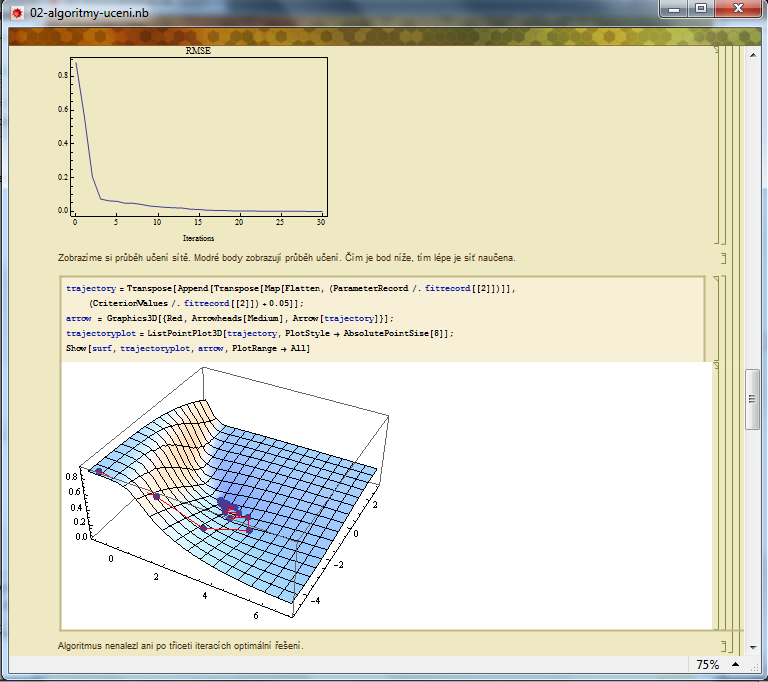
\includegraphics[height=10cm]{figures/ukazka02.png}
\caption{Ukázka souboru 02-algoritmy-uceni.nb}
\label{fig:algoritmy-uceni}
\end{center}
\end{figure}
\newpage
\section{Křížová validace}
V kapitole křížová validace seznamuji studenty s principem fungování křížové validace. Křížovou validaci ukazuji na Iris datech a jednoduché dopředné síti.

Nejprve jsem načetl data. Iris data jsem rozdělil na vstupní a výstupní vektory, výstupní vektory jsem zakódoval kódem 1 z N. Poté detailně rozebral předzpracování dat pro křížovou validaci. Dále jsem vytvořil neuronovou síť, kterou jsem pomocí křížové validace testoval. Následně jsem naimplementoval samotnou křížovou validaci. V této implementaci jsem vypisoval pro každý fold úspěšnost RMSE, kterou síť dosáhla. Po skončení všech kol křížové validace jsem zobrazil boxový graf s výsledky křížové validace viditelný na obrázku~\ref{fig:krossvalidace}. Po najetí myší na graf se k němu zobrazí legenda. Studenti jsem dal také možnost nechat si vypsat výsledky křížové validace v textovém formátu. Textový formát vypíše nejlepší výsledek, nejhorší výsledek a aritmetický průměr všech výsledků. Na závěr jsem dal studentům možnost provést si křížovou validaci vlastní sítě s vlastními daty. Vlastní křížové validaci nastaví student parametry jednoduchým přiřazením do proměnných, je potřeba aby  zadaná síť odpovídala zadaným vstupním a výstupním datům a data byla předzpracována pomocí postupu uvedeného v této kapitole. Tato kapitola se nachází v souboru \textit{03-krossvalidace.nb}.

\begin{figure}[h!]
\begin{center}
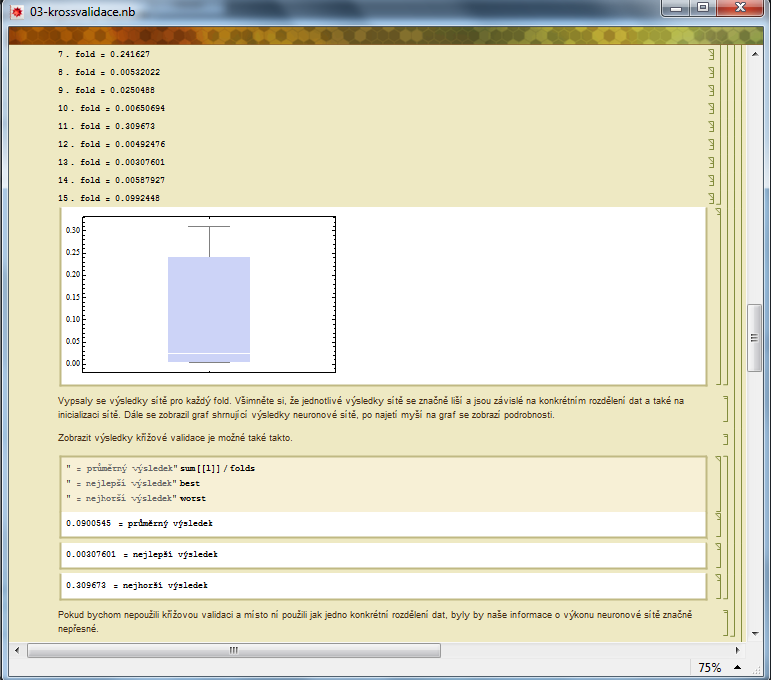
\includegraphics[height=10cm]{figures/ukazka03.png}
\caption{Ukázka souboru 03-krossvalidace.nb}
\label{fig:krossvalidace}
\end{center}
\end{figure}

\section{Dopředná síť}
\subsection{Jednoduchá data sin(x)}
V této kapitole poprvé seznamuji studenty s dopřednou neuronovou sítí. Funkci dopředné neuronové sítě jsem demonstroval na aproximaci funkce sinus.

Nejprve jsem připravil jednoduchá trénovací data navzorkováním funkce sinus na intervalu <0, 2\begin{math}\pi \end{math}>. Navzorkovaná data jsem pro jasnou představu zobrazil v textové i grafické podobě. Poté jsem ukázal jakým způsobem vytvořit neuronovou síť požadované struktury, jak si zobrazit dodatečné informace o síti a jak síť naučit na trénovacích datech. Dále jsem graficky zobrazil výstup sítě před naučením a po naučení jak je vidět na obrázku~\ref{fig:feedforward-sin}. Na závěr jsem ukázal jak převést síť do formy vzorce. Tato kapitola se nachází v souboru \textit{04-feedforward-sin.nb}.

\begin{figure}[h!]
\begin{center}
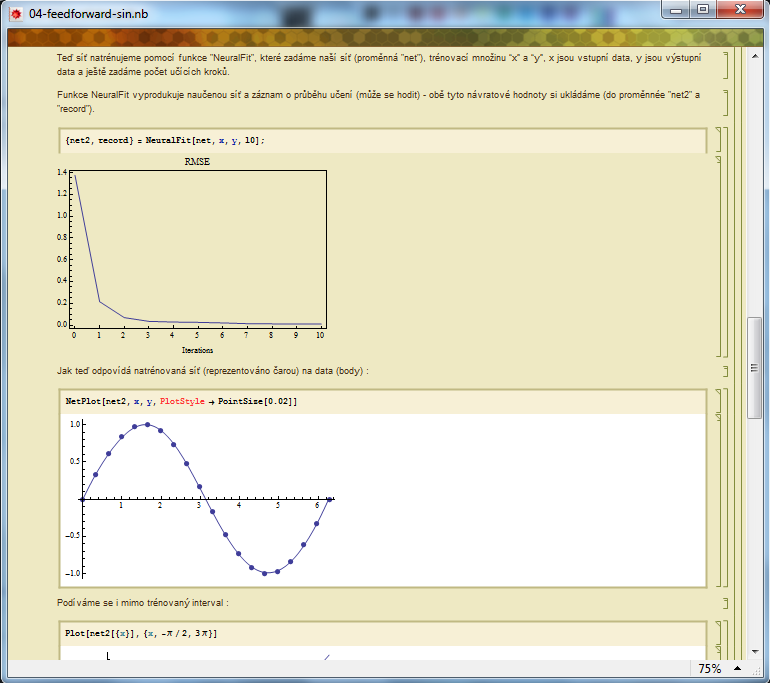
\includegraphics[height=10cm]{figures/ukazka04.png}
\caption{Ukázka souboru 04-feedforard-sin.nb}
\label{fig:feedforward-sin}
\end{center}
\end{figure}

Soubor vznikl úpravou souboru Petra Chlumského. Změnil jsem vzhled notebooku a upravil doprovodný komentář.

\subsection{Iris data}
V této kapitole ukazuji jakým způsobem pomocí dopředné sítě klasifikovat Iris data.

Nejprve jsem načetl data. Studentům jsme dal na výběr zda chtějí načíst data z internetu nebo použít lokální soubor s daty. Poté jsem data předzpracoval. Data jsem rozdělil na vstupní a výstupní vektory, protože výstupní parametr je textový, provedl jsem jeho překódování metodou 1 z N, kdy je každé třídě přiřazen jeden výstupní vektor. Toto předzpracování jsem prováděl krok po kroku s velmi podrobným komentářem a ještě jsem ho doplnil několika dalšími ukázkovými příklady. Po předzpracování dat jsem vytvořil dopřednou neuronovou síť, a data jsem touto neuronovou sítí zpracoval. Dále jsem zobrazil jak se vyvíjela úspěšnost klasifikace v průběhu učení (zobrazeno na obrázku~\ref{fig:feedforward-iris}). Na závěr jsem použil 3D graf, který ukazuje úspěšnost sítě na trénovacích datech (také ukázáno na obrázku~\ref{fig:feedforward-iris}). Také jsem ukázal možnost jak síť nechat symbolicky vyhodnotit. Tato kapitola se nachází v souboru \textit{05-feedforward-iris.nb}.

\begin{figure}[h!]
\begin{center}
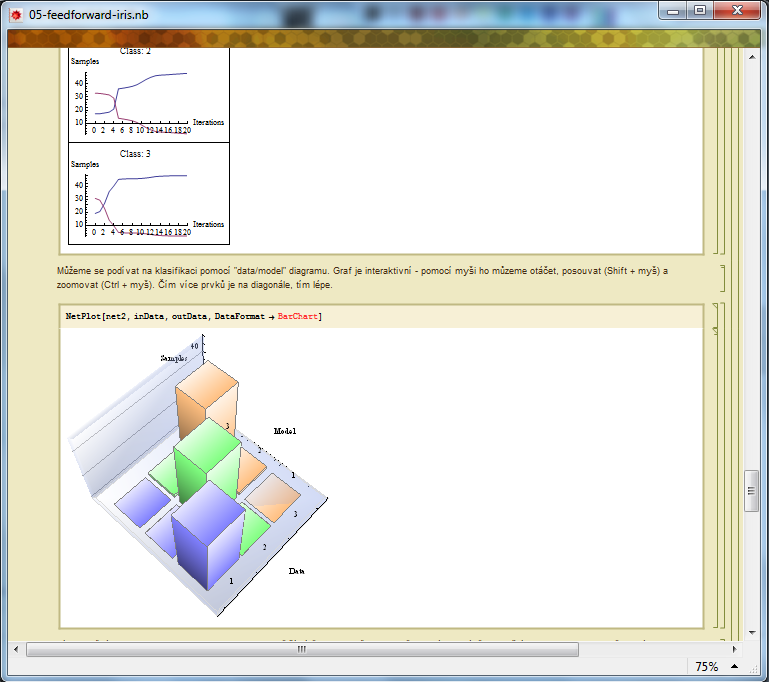
\includegraphics[height=10cm]{figures/ukazka05.png}
\caption{Ukázka souboru 05-feedforard-iris.nb}
\label{fig:feedforward-iris}
\end{center}
\end{figure}

Soubor vznikl úpravou souboru Petra Chlumského. Změnil jsem vzhled notebooku. V doprovodném komentáři jsem nahradil sousloví \uv{skupina v datech} slovem \uv{třída}, které podle mého názoru lépe vystihuje popisovanou skutečnost. Dále jsem komentář rozšířil. V závěru notebooku jsem nezobrazoval vývoj úspěšnosti klasifikace během učení ve 3D grafu, který podle mě nebyl tak přehledný a jasný jako 2D graf, který je zobrazen.

\subsection{Různé přístupy k učení sítě}
V tomto notebooku ukazuji několik různých přístupů k učení dopředné sítě. Tyto přístupy se liší hlavně v dělení dat na trénovací, testovací a validační množinu. Ukazuji také použití křížové validace a rozebírám vyhodnocení úspěšnosti neuronové sítě.

Nejprve jsem načetl Iris data a provedl jejich předzpracování stejně jako v minulé kapitole. Takto předzpracovaná data jsem náhodně rozdělil na trénovací, validační a testovací množinu. Ukázal jsem možnost použití křížové validace k určení vhodné struktury sítě. Při křížové validaci jsem výsledky sítí porovnával podle hodnoty RMSE, výsledky křížové validace jsem zobrazil v boxovém grafu, který je na obrázku~\ref{fig:feedforward-iris-2}. Síť, která vyšla z křížové validace nejlépe, jsem poté naučil na trénovací množině s použitím validační množiny. Validační množinu jsem použil k zastavení učení sítě, pokud by se úspěšnost klasifikace na validační množině začala v průběhu učení zhoršovat. Poté jsem vyhodnotil úspěšnost klasifikace na testovací množině. Tuto úspěšnost jsem pro snadnou čitelnost uvedl v procentech. Dále jsem síť se stejnou strukturou naučil bez použití validační množiny a taktéž jsem vyhodnotil její úspěšnost. Kapitola se nachází v souboru \textit{06-feedforward-iris-2}.

\begin{figure}[h!]
\begin{center}
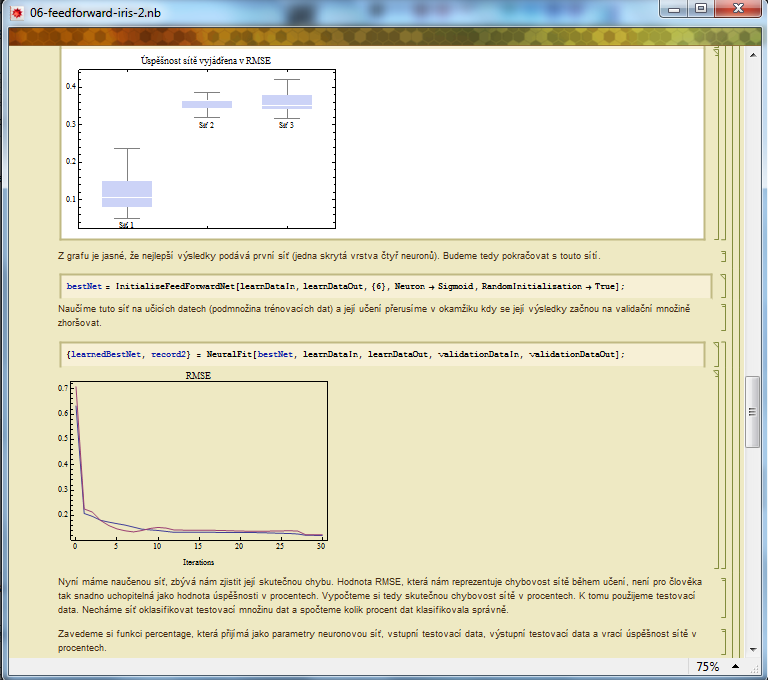
\includegraphics[height=10cm]{figures/ukazka06.png}
\caption{Ukázka souboru 06-feedforard-iris-2.nb}
\label{fig:feedforward-iris-2}
\end{center}
\end{figure}

\section{RBF síť}
\subsection{Ukázka výstupu skrytého neuronu}
Tato kapitola není určena přímo pro experimentování se sítí, ale spíše pro pochopení jakým způsobem RBF síť funguje. V notebooku zobrazuji výstup skrytého RBF neuronu.

Nejprve jsem vygeneroval vstupní data. Data jsou tvořena dvěma dobře oddělenými shluky, každý shluk představuje jednu třídu. Poté jsem vytvořil jednoduchou RBF neuronovou síť s jedním skrytým RBF neuronem, pomocí které jsem vstupní data klasifikoval. Síť jsem naučil na vygenerovaných datech, poté jsem zobrazil výstup RBF neuronu. Pro lepší představu o tom, jakým způsobem RBF neuron pokryl vstupní data, jsem tato data zobrazil společně s výstupem neuronu do jednoho grafu, který je na obrázku~\ref{fig:rbf-neuron}. Kapitola se nachází v souboru \textit{07-rbf-neuron.nb}.

\begin{figure}[h!]
\begin{center}
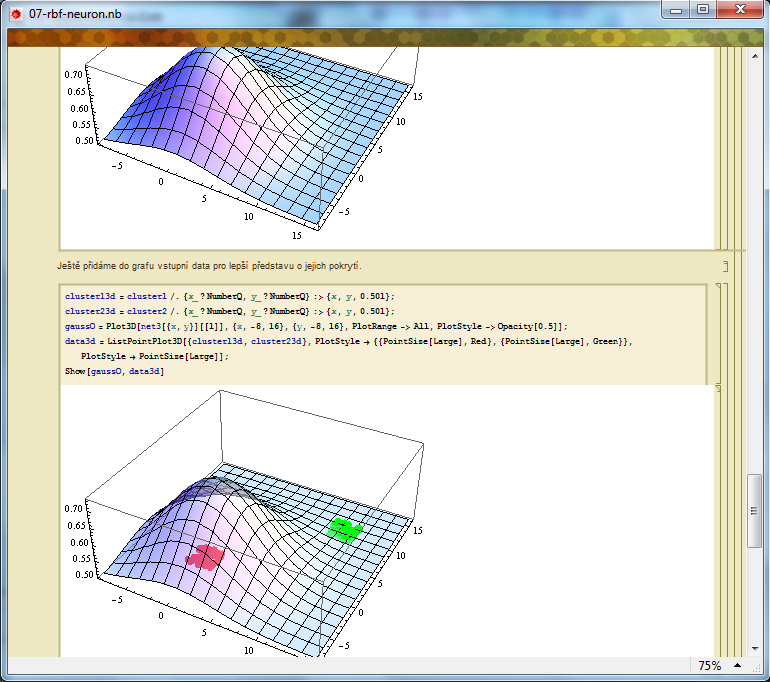
\includegraphics[height=10cm]{figures/ukazka07.png}
\caption{Ukázka souboru 07-rbf-neuron.nb}
\label{fig:rbf-neuron}
\end{center}
\end{figure}

\subsection{Ukázka výstupu tří skrytých neuronů}
Tato kapitola, stejně jako předchozí, slouží primárně k pochopení fungování RBF sítě. V notebooku zobrazuji výstup skryté vrstvy neuronů u RBF sítě se třemi RBF neurony, která je naučena na složitějších datech. 

Nejprve jsem vygeneroval data. Data se skládají ze šesti oddělených shluků, obsahují dvě třídy, každá třída se skládá ze třech shluků. Data jsem pro představu zobrazil v grafu. Dále jsem vytvořil RBF neuronovou síť, kterou jsem chtěl vygenerovaná data klasifikovat. Síť jsem naučil na vygenerovaných datech. Poté jsem zobrazil výstup neuronové sítě ve 2D i 3D grafu (zobrazeno na obrázku~\ref{fig:rbf-neuron2}), na kterých ukazuji jak síť klasifikuje data. Poté jsem zobrazen výstup skryté vrstvy RBF neuronů. Do stejného grafu s výstupem jednotlivých RBF neuronů jsem zobrazil i vstupní data, aby bylo vidět jak se RBF neurony přizpůsobily datům. Kapitola je v souboru \textit{08-rbf-neuron-2.nb}.

\begin{figure}[h!]
\begin{center}
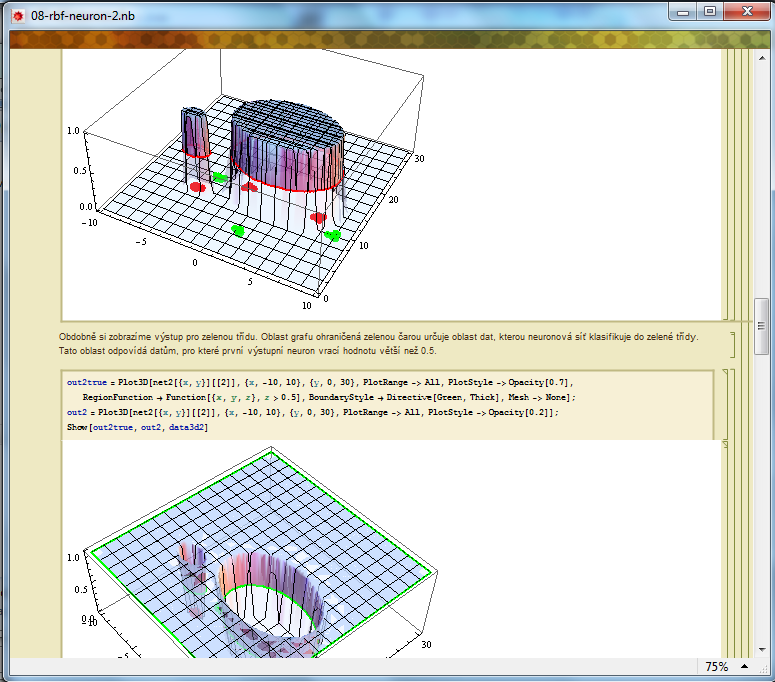
\includegraphics[height=10cm]{figures/ukazka08.png}
\caption{Ukázka souboru 08-rbf-neuron-2.nb}
\label{fig:rbf-neuron2}
\end{center}
\end{figure}

\subsection{Jednoduchá data sin(x)}
V této kapitole poprvé seznamuji studenty s RBF sítí. Ukazuji jak pomocí RBF sítě zpracovat jednoduchá data, v tomto případě se jedná o aproximaci funkce sinus.

Nejprve jsem vygeneroval data navzorkováním funkce sinus na intervalu <0, 2\begin{math}\pi \end{math}>. Data jsem zobrazil v grafické i textové podobě, aby o nich měli studenti dobrou představu. Dále jsem ukázal jak vytvořit RBF neuronovou síť požadované struktury, jak si o ní zobrazit podrobnější informace a jakým způsobem jí naučit na trénovacích datech. Dále ukazuji jak reagovala nenaučená síť (je vidět na obrázku~\ref{fig:rbf-sin}) na data a také jak reaguje naučená síť na stejná data. Na závěr jsem ukázal jak je možné nechat síť symbolicky vyhodnotit (zobrazit ji ve formě vzorce). Kapitola je v souboru \textit{09-rbf-sin.nb}.

\begin{figure}[h!]
\begin{center}
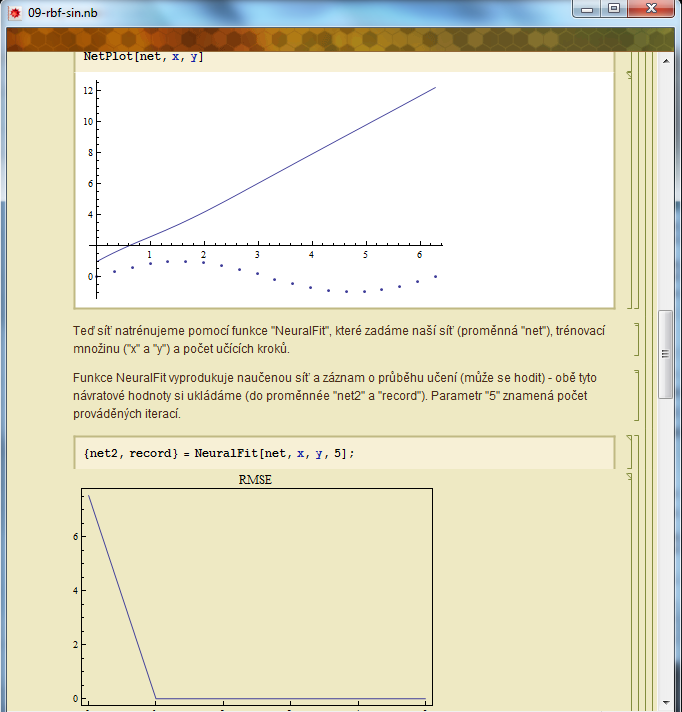
\includegraphics[height=10cm]{figures/ukazka09.png}
\caption{Ukázka souboru 09-rbf-sin.nb}
\label{fig:rbf-sin}
\end{center}
\end{figure}

Soubor vznikl úpravou souboru Petra Chlumského. Změnil jsem vzhled a rozšířil doprovodný komentář. Dále jsem odstranil nepřesné a nepravdivé popisky u vytváření RBF sítě a nahradil je správnou verzí.
\newpage
\subsection{Iris data}
Touto kapitolou ukazuji zpracování složitějších dat neuronovou sítí RBF. V notebooku provádím klasifikování Iris dat z UCI databáze \cite{UCI}.

Nejprve jsem načetl Iris data (opět jsem dal na výběr za je načíst ze souboru nebo z internetu), poté jsem provedl rozdělení dat na vstupní a výstupní vektory a výstupní data jsem zakódoval algoritmem 1 z N. Dále jsem vytvořil RBF síť, která jsem následně naučil na datech. Potom jsem zobrazil graf, který ukazuje jak se vyvíjela úspěšnost klasifikace v průběhu učení. Níže jsem ještě vykreslil graf porovnávající zadaná data s výstupem naší naučené RBF sítě. Na závěr jsem ukázal možnost symbolického vyhodnocení sítě. Kapitolu naleznete v souboru \textit{10-rbf-iris.nb}.

Soubor vznikl úpravou souboru Petra Chlumského. Změnil jsem grafický vzhled notebooku. Dále jsem významně zkrátil sekci předzpracování dat. V původním notebooku bylo předzpracování stejně rozsáhlé jako v souboru \textit{05-feedforward-iris.nb}, já ponechal pouze kód, který skutečně zpracovává Iris data a uvedl odkaz na soubor ve kterém je předzpracování popsáno podrobněji. Dále jsem na závěr notebooku nezobrazoval 3D graf s vývojem úspěšnosti klasifikace, který podle mého názoru není tolik vypovídající. Ponechal jsem 2D graf s vývojem klasifikace. Také jsem rozšířil komentář a opravil špatný popis u vytváření RBF sítě.
\subsection{Různé přístupy k učení sítě}
Kapitolou chci demonstrovat různé možnosti jak přistoupit k učení RBF sítě z hlediska rozdělení dat na trénovací, testovací a validační množinu. Také ukazuji možnost využití křížové validace k určení nejvhodnější struktury sítě. Na závěr ukazuji jak vyhodnotit úspěšnost sítě.

Nejprve jsem načetl Iris data (v notebooku jsem dal na výběr zda  ze souboru nebo z internetu). Načtená data jsem rozdělil na vstupní a výstupní vektory, výstupní vektory jsem překódoval kódem 1 z N. Takto zpracovaná data jsem rozdělil na trénovací, testovací a validační množinu. Dále jsem demonstroval možnost použití křížové validace, k určení nejvhodnější struktury sítě (v tomto případě k určení počtu RBF neuronů). Výsledek křížové validace jsem zobrazil v boxovém grafu. Dále jsem ukázal možnost učení RBF sítě s validační množinou. Validační množina slouží ke kontrole úspěšnosti sítě, jakmile se výsledky na validační množině zhorší oproti předchozí iteraci, je učení sítě ukončeno. Na testovacích datech jsem poté provedl určení skutečné úspěšnosti naučené sítě, kterou jsem vyjádřil v procentech. Dále jsem ukázal učení sítě bez použití validační množiny. U takto naučené sítě jsem také určil skutečnou úspěšnost na testovacích datech v procentech. Kapitola se nachází v souboru \textit{11-rbf-iris-2.nb}.
\section{Hopfieldova síť}
V této kapitole představuji studentům Hopfieldovou neuronovou síť a ukazuji její použití na jednoduchých datech.

Jako vstupní data jsem použil obrázky číslic 1, 2 a 3 zobrazené v poli 8x8, kde černá znamená 1 a bílá -1. Zobrazení dat můžete vidět na obrázku~\ref{fig:hopfield}. Tato data jsem zadal přímo v kódu. Poté jsem vytvořil Hopfieldovu síť, která jsem následně na vstupních datech naučil. Pro otestování, jak síť reaguje na data jsem potřeboval vytvořit testovací data, ta jsem vytvořil aplikací šumu na vstupní data. Tato zašuměná data jsem předložil naučené síti a zobrazil její reakci na ně. Na závěr jsem zobrazil graf ukazující jakým způsobem se minimalizovala energetická funkce pro jednotlivé předložené vzory. Kapitola se nalézá v souboru \textit{12-hopfield.nb}.

\begin{figure}[h!]
\begin{center}
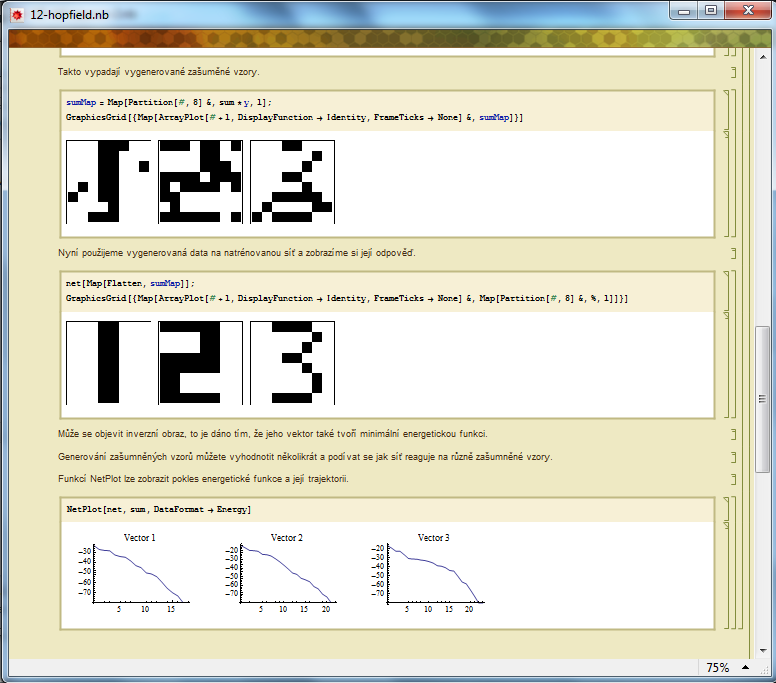
\includegraphics[height=10cm]{figures/ukazka12.png}
\caption{Ukázka souboru 12-hopfield.nb}
\label{fig:hopfield}
\end{center}
\end{figure}

Soubor vznikl úpravou souboru Petra Chlumského. Mimo úpravy celkového vzhledu notebooku a drobných úprav doprovodného komentáře spočívá hlavní úprava v nahrazení funkce GraphicsArray funkcí GraphicsGrid. Funkce GraphicsArray je v Mathematice 8 zastaralá a nedoporučuje se používat. Také jsem upravil funkci pro aplikaci šumu, která nyní zašumí předložený vzor o trochu více než tomu bylo dříve.
\newpage
\section{Samoorganizující mapy}
\subsection{Shlukování dat}
V této kapitole seznamuji studenty se samoorganizující se mapou a ukazuji její použití na jednoduchých datech. Pomocí samoorganizující se mapy hledám shluky ve vygenerovaných datech.

Na začátku jsem vygeneroval vstupní data. Data obsahují šest dobře oddělených shluků. V těchto datech jsem hledal pomocí samoorganizující se mapy šest shluků. Nejprve jsem vytvořil náhodně inicializovanou samoorganizující se mapu, kterou jsem naučil na vstupních datech. Pomocí grafu jsem zobrazil její výstup (tedy jak síť rozdělila data na shluky). Dále jsem ukázal jak odstranit ze sítě nepotřebný (mrtvý) neuron a zobrazil jsem výstup sítě bez nepotřebného neuronu. Následně jsem ukázal postup umožňující dosažení lepších výsledků. Samoorganizující se mapa jsem neinicializoval náhodně, ale použil jsem k její inicializaci metodou SOM. Poté jsem síť doučil na vstupních datech a graficky zobrazil její výstup, který je zobrazen na obrázku~\ref{fig:som-clustering}. Na závěr jsem zobrazil průběh učení obou sítí. Nejprve ve formě statického grafu, který zobrazuje trajektorii jednotlivých neuronů v průběhu učení. Podruhé jako interaktivní graf zobrazující výstup sítě pro danou iteraci. Pomocí posuvníku je možné vybírat, která iterace je zobrazena. Kapitola se nachází v souboru \textit{13-som-clustering.nb}.

\begin{figure}[h!]
\begin{center}
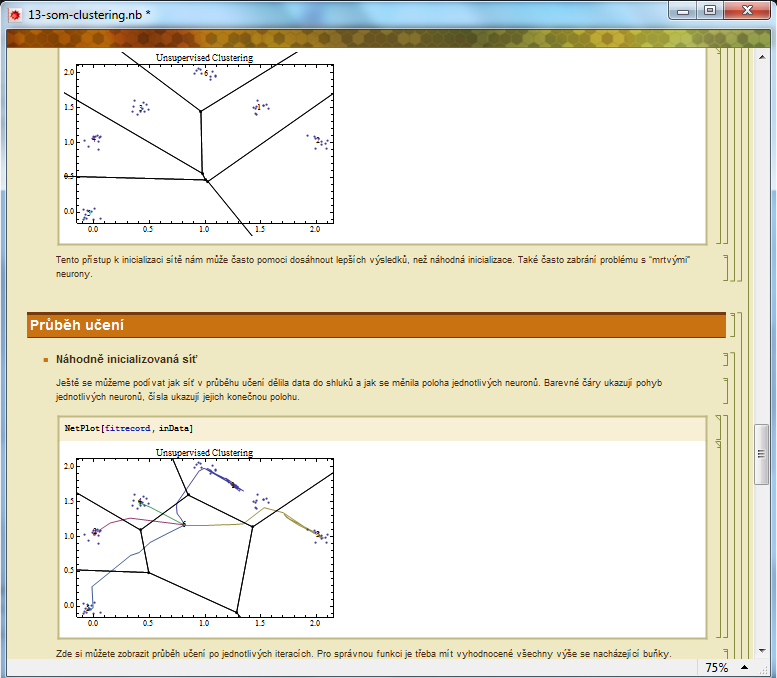
\includegraphics[height=10cm]{figures/ukazka13.png}
\caption{Ukázka souboru 13-som-clustering.nb}
\label{fig:som-clustering}
\end{center}
\end{figure}

\subsection{SOM a Iris data}
Touto kapitolou demonstruji použití samoorganizující se mapy na složitějších datech. K ukázce použití jsem z zvolil Iris data.

Nejprve jsem načetl Iris data(studentům jsem dal možnost načtení ze souboru nebo z internetu). Data jsem rozdělil na vstupní a výstupní vektory, výstupní vektory jsem překódoval metodou 1 z N. Dále jsem vytvořil samoorganizující se mapu, kterou jsem naučil na vstupních datech. Tento graf můžete vidět na obrázku~\ref{fig:som-iris}. Poté jsem vykreslil graf, který zobrazuje kolik vektorů náleží ke každému neuronu v síti. Stejným způsobem jsem zobrazil i průběh učení sítě. Následně jsem ukázal jakým způsobem lze libovolnému vektoru přiřadit jeho reprezentanta, jak spočítat Eukleidovskou vzdálenost od reprezentanta a také jsem připomněl mazání nepotřebných neuronů. Na závěr jsem rozebral doučování sítě. Kapitola se nalézá v souboru \textit{14-som-iris.nb}.

\begin{figure}[h!]
\begin{center}
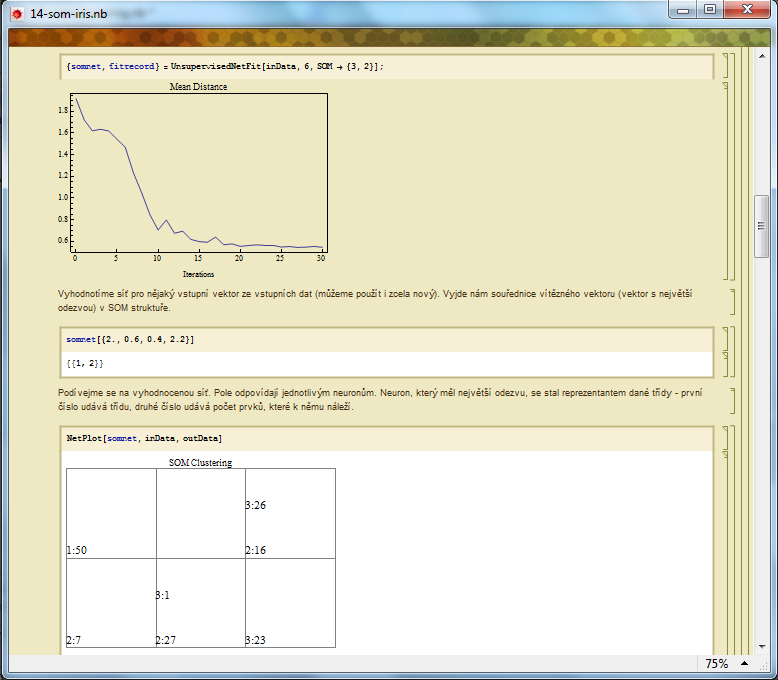
\includegraphics[height=10cm]{figures/ukazka14.png}
\caption{Ukázka souboru 14-som-iris.nb}
\label{fig:som-iris}
\end{center}
\end{figure}

Soubor vznikl úpravou souboru Petra Chlumského. Změnil jsem celkový vzhled notebooku, v komentáři jsem nahradil slovo \uv{skupina} slovem \uv{třída}, které podle mě lépe vystihuje popisovanou věc. Udělal jsem ještě několik menších úprav a rozšíření v komentáři. Dále jsem provedl úpravu předzpracování dat, které bylo zbytečně rozsáhlé a tím pádem zdlouhavé. Ponechal jsem pouze minimální potřebný kód a uvedl odkaz na notebook ve kterém je předzpracování dat detailně popsáno.
\section{LVQ}
V poslední kapitole seznamuji studenty s použitím LVQ sítě. Použití LVQ sítě je ukázáno na klasifikaci Iris dat.

Nejprve jsem načetl Iris data (dávám možnost načtení ze souboru nebo z internetu), data jsem rozdělil na vstupní a výstupní vektory a výstupní vektory jsem překódoval metodou 1 z N. Nejprve jsem nabídl několik pohledů na vstupní data (jeden z nich je na obrázku~\ref{fig:lvq}, společně s vytvořením LVQ sítě), poté jsem vytvořil LVQ síť, kterou jsem naučil na vstupních datech. Poté jsem zobrazil vizualizaci výstupu sítě v průběhu učení. Následně jsem ukázal jakým způsobem smazat nepotřebné neurony. Dále jsem demonstroval jak je možné nechat oklasifikovat libovolný vektor. Poté jsem zobrazil procentuální úspěšnost klasifikace. Na závěr jsem rozebral možnosti doučování sítě a ukázal několik možných grafických výstupů sítě. Tato kapitola se nachází v souboru \textit{15-lvq-iris.nb}.

\begin{figure}[h!]
\begin{center}
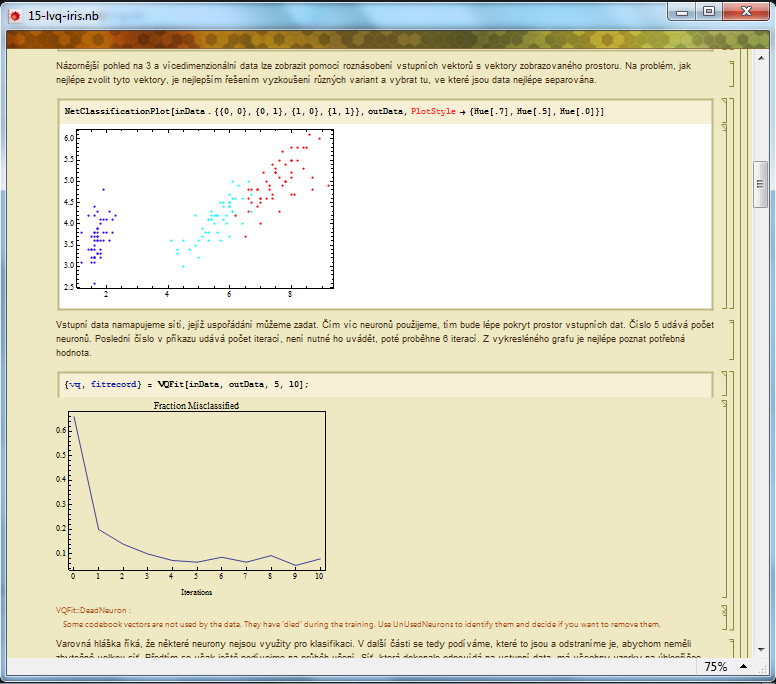
\includegraphics[height=10cm]{figures/ukazka15.png}
\caption{Ukázka souboru 15-lvq.nb}
\label{fig:lvq}
\end{center}
\end{figure}

Soubor vznikl úpravou souboru Petra Chlumského. Změnil jsem grafickou podobu notebooku. V doprovodném komentáři jsem nahradil slovo \uv{skupina} slovem \uv{třída}, které lépe vystihuje popisovanou skutečnost. Komentář jsem ještě drobně rozšířil a upravil. Upravil jsem a výrazně zkrátil předzpracování dat. Ponechal jsem pouze kód, který skutečně manipuluje s daty a uvedl odkaz na notebook, ve kterém se nachází detailně popsaný proces předzpracování dat. 
%*****************************************************************************
\chapter{Závěr}

\begin{itemize}
\item Zhodnocení splnění cílů DP/BP a  vlastního přínosu práce (při formulaci je třeba vzít v potaz zadání práce).
\item Diskuse dalšího možného pokračování práce.
\end{itemize} 

%*****************************************************************************
% Seznam literatury je v samostatnem souboru reference.bib. Ten
% upravte dle vlastnich potreb, potom zpracujte (a do textu
% zapracujte) pomoci prikazu bibtex a nasledne pdflatex (nebo
% latex). Druhy z nich alespon 2x, aby se poresily odkazy.

% originally following specification for bibliography formating was used
%\bibliographystyle{abbrv}

% Here is an improvment by Petr Dlouhy (April 2010).
% It is mainly for supervisors who expect Czech fomrating rules for references
% Additional feature is live url addresses to sources from your pdf file
% It requires the file csplainnat.bst (included in this sample zipfile).

\bibliographystyle{csplainnat}

%bibliographystyle{plain}
%\bibliographystyle{psc}
{
%JZ: 11.12.2008 Kdo chce mit v techto ukazkovych odkazech take odkaz na CSTeX:
\def\CS{$\cal C\kern-0.1667em\lower.5ex\hbox{$\cal S$}\kern-0.075em $}
\bibliography{reference}
}

% M. Dušek radi:
%\bibliographystyle{alpha}
% kdy citace ma tvar [AutorRok] (napriklad [Cook97]). Sice to asi neni  podle ceske normy (BTW BibTeX stejne neodpovida ceske norme), ale je to nejprehlednejsi.
% 3.5.2009 JZ polemizuje: BibTeX neobvinujte, napiste a poskytnete nam styl (.bst) splnujici citacni normu CSN/ISO.

%*****************************************************************************
%*****************************************************************************
\appendix

\chapter{Testování zaplnění stránky a odsazení odstavců}
\textbf{\large Tato příloha nebude součástí vaší práce. 
Slouží pouze jako příklad formátování textu.}

\section*{}
Určitě existuje nějaká pěkná latinská věta, která se k tomuhle testování používá, ale co mají dělat ti, kteří se nikdy latinsky neučili? Určitě existuje nějaká pěkná latinská věta, která se k tomuhle testování používá, ale co mají dělat ti, kteří se nikdy latinsky neučili? Určitě existuje nějaká pěkná latinská věta, která se k tomuhle testování používá, ale co mají dělat ti, kteří se nikdy latinsky neučili?

Určitě existuje nějaká pěkná latinská věta, která se k tomuhle testování používá, ale co mají dělat ti, kteří se nikdy latinsky neučili? Určitě existuje nějaká pěkná latinská věta, která se k tomuhle testování používá, ale co mají dělat ti, kteří se nikdy latinsky neučili? Určitě existuje nějaká pěkná latinská věta, která se k tomuhle testování používá, ale co mají dělat ti, kteří se nikdy latinsky neučili?

Určitě existuje nějaká pěkná latinská věta, která se k tomuhle testování používá, ale co mají dělat ti, kteří se nikdy latinsky neučili? Určitě existuje nějaká pěkná latinská věta, která se k tomuhle testování používá, ale co mají dělat ti, kteří se nikdy latinsky neučili? Určitě existuje nějaká pěkná latinská věta, která se k tomuhle testování používá, ale co mají dělat ti, kteří se nikdy latinsky neučili?

Určitě existuje nějaká pěkná latinská věta, která se k tomuhle testování používá, ale co mají dělat ti, kteří se nikdy latinsky neučili? Určitě existuje nějaká pěkná latinská věta, která se k tomuhle testování používá, ale co mají dělat ti, kteří se nikdy latinsky neučili? Určitě existuje nějaká pěkná latinská věta, která se k tomuhle testování používá, ale co mají dělat ti, kteří se nikdy latinsky neučili? Určitě existuje nějaká pěkná latinská věta, která se k tomuhle testování používá, ale co mají dělat ti, kteří se nikdy latinsky neučili? Určitě existuje nějaká pěkná latinská věta, která se k tomuhle testování používá, ale co mají dělat ti, kteří se nikdy latinsky neučili? Určitě existuje nějaká pěkná latinská věta, která se k tomuhle testování používá, ale co mají dělat ti, kteří se nikdy latinsky neučili?

Určitě existuje nějaká pěkná latinská věta, která se k tomuhle testování používá, ale co mají dělat ti, kteří se nikdy latinsky neučili? Určitě existuje nějaká pěkná latinská věta, která se k tomuhle testování používá, ale co mají dělat ti, kteří se nikdy latinsky neučili?

Určitě existuje nějaká pěkná latinská věta, která se k tomuhle testování používá, ale co mají dělat ti, kteří se nikdy latinsky neučili? Určitě existuje nějaká pěkná latinská věta, která se k tomuhle testování používá, ale co mají dělat ti, kteří se nikdy latinsky neučili? Určitě existuje nějaká pěkná latinská věta, která se k tomuhle testování používá, ale co mají dělat ti, kteří se nikdy latinsky neučili? Určitě existuje nějaká pěkná latinská věta, která se k tomuhle testování používá, ale co mají dělat ti, kteří se nikdy latinsky neučili? Určitě existuje nějaká pěkná latinská věta, která se k tomuhle testování používá, ale co mají dělat ti, kteří se nikdy latinsky neučili?

Určitě existuje nějaká pěkná latinská věta, která se k tomuhle testování používá, ale co mají dělat ti, kteří se nikdy latinsky neučili? Určitě existuje nějaká pěkná latinská věta, která se k tomuhle testování používá, ale co mají dělat ti, kteří se nikdy latinsky neučili? Určitě existuje nějaká pěkná latinská věta, která se k tomuhle testování používá, ale co mají dělat ti, kteří se nikdy latinsky neučili? Určitě existuje nějaká pěkná latinská věta, která se k tomuhle testování používá, ale co mají dělat ti, kteří se nikdy latinsky neučili? Určitě existuje nějaká pěkná latinská věta, která se k tomuhle testování používá, ale co mají dělat ti, kteří se nikdy latinsky neučili?

Určitě existuje nějaká pěkná latinská věta, která se k tomuhle testování používá, ale co mají dělat ti, kteří se nikdy latinsky neučili? Určitě existuje nějaká pěkná latinská věta, která se k tomuhle testování používá, ale co mají dělat ti, kteří se nikdy latinsky neučili? Určitě existuje nějaká pěkná latinská věta, která se k tomuhle testování používá, ale co mají dělat ti, kteří se nikdy latinsky neučili? Určitě existuje nějaká pěkná latinská věta, která se k tomuhle testování používá, ale co mají dělat ti, kteří se nikdy latinsky neučili? Určitě existuje nějaká pěkná latinská věta, která se k tomuhle testování používá, ale co mají dělat ti, kteří se nikdy latinsky neučili?

Určitě existuje nějaká pěkná latinská věta, která se k tomuhle testování používá, ale co mají dělat ti, kteří se nikdy latinsky neučili? Určitě existuje nějaká pěkná latinská věta, která se k tomuhle testování používá, ale co mají dělat ti, kteří se nikdy latinsky neučili? Určitě existuje nějaká pěkná latinská věta, která se k tomuhle testování používá, ale co mají dělat ti, kteří se nikdy latinsky neučili? Určitě existuje nějaká pěkná latinská věta, která se k tomuhle testování používá, ale co mají dělat ti, kteří se nikdy latinsky neučili? Určitě existuje nějaká pěkná latinská věta, která se k tomuhle testování používá, ale co mají dělat ti, kteří se nikdy latinsky neučili?

Určitě existuje nějaká pěkná latinská věta, která se k tomuhle testování používá, ale co mají dělat ti, kteří se nikdy latinsky neučili? Určitě existuje nějaká pěkná latinská věta, která se k tomuhle testování používá, ale co mají dělat ti, kteří se nikdy latinsky neučili? Určitě existuje nějaká pěkná latinská věta, která se k tomuhle testování používá, ale co mají dělat ti, kteří se nikdy latinsky neučili? Určitě existuje nějaká pěkná latinská věta, která se k tomuhle testování používá, ale co mají dělat ti, kteří se nikdy latinsky neučili? Určitě existuje nějaká pěkná latinská věta, která se k tomuhle testování používá, ale co mají dělat ti, kteří se nikdy latinsky neučili?

Určitě existuje nějaká pěkná latinská věta, která se k tomuhle testování používá, ale co mají dělat ti, kteří se nikdy latinsky neučili? Určitě existuje nějaká pěkná latinská věta, která se k tomuhle testování používá, ale co mají dělat ti, kteří se nikdy latinsky neučili? Určitě existuje nějaká pěkná latinská věta, která se k tomuhle testování používá, ale co mají dělat ti, kteří se nikdy latinsky neučili? Určitě existuje nějaká pěkná latinská věta, která se k tomuhle testování používá, ale co mají dělat ti, kteří se nikdy latinsky neučili? Určitě existuje nějaká pěkná latinská věta, která se k tomuhle testování používá, ale co mají dělat ti, kteří se nikdy latinsky neučili?

Určitě existuje nějaká pěkná latinská věta, která se k tomuhle testování používá, ale co mají dělat ti, kteří se nikdy latinsky neučili? Určitě existuje nějaká pěkná latinská věta, která se k tomuhle testování používá, ale co mají dělat ti, kteří se nikdy latinsky neučili? Určitě existuje nějaká pěkná latinská věta, která se k tomuhle testování používá, ale co mají dělat ti, kteří se nikdy latinsky neučili? Určitě existuje nějaká pěkná latinská věta, která se k tomuhle testování používá, ale co mají dělat ti, kteří se nikdy latinsky neučili? Určitě existuje nějaká pěkná latinská věta, která se k tomuhle testování používá, ale co mají dělat ti, kteří se nikdy latinsky neučili?

Určitě existuje nějaká pěkná latinská věta, která se k tomuhle testování používá, ale co mají dělat ti, kteří se nikdy latinsky neučili? Určitě existuje nějaká pěkná latinská věta, která se k tomuhle testování používá, ale co mají dělat ti, kteří se nikdy latinsky neučili? Určitě existuje nějaká pěkná latinská věta, která se k tomuhle testování používá, ale co mají dělat ti, kteří se nikdy latinsky neučili? Určitě existuje nějaká pěkná latinská věta, která se k tomuhle testování používá, ale co mají dělat ti, kteří se nikdy latinsky neučili? Určitě existuje nějaká pěkná latinská věta, která se k tomuhle testování používá, ale co mají dělat ti, kteří se nikdy latinsky neučili?

Určitě existuje nějaká pěkná latinská věta, která se k tomuhle testování používá, ale co mají dělat ti, kteří se nikdy latinsky neučili? Určitě existuje nějaká pěkná latinská věta, která se k tomuhle testování používá, ale co mají dělat ti, kteří se nikdy latinsky neučili? Určitě existuje nějaká pěkná latinská věta, která se k tomuhle testování používá, ale co mají dělat ti, kteří se nikdy latinsky neučili? Určitě existuje nějaká pěkná latinská věta, která se k tomuhle testování používá, ale co mají dělat ti, kteří se nikdy latinsky neučili? Určitě existuje nějaká pěkná latinská věta, která se k tomuhle testování používá, ale co mají dělat ti, kteří se nikdy latinsky neučili?

Určitě existuje nějaká pěkná latinská věta, která se k tomuhle testování používá, ale co mají dělat ti, kteří se nikdy latinsky neučili? Určitě existuje nějaká pěkná latinská věta, která se k tomuhle testování používá, ale co mají dělat ti, kteří se nikdy latinsky neučili? Určitě existuje nějaká pěkná latinská věta, která se k tomuhle testování používá, ale co mají dělat ti, kteří se nikdy latinsky neučili? Určitě existuje nějaká pěkná latinská věta, která se k tomuhle testování používá, ale co mají dělat ti, kteří se nikdy latinsky neučili? Určitě existuje nějaká pěkná latinská věta, která se k tomuhle testování používá, ale co mají dělat ti, kteří se nikdy latinsky neučili?

Určitě existuje nějaká pěkná latinská věta, která se k tomuhle testování používá, ale co mají dělat ti, kteří se nikdy latinsky neučili? Určitě existuje nějaká pěkná latinská věta, která se k tomuhle testování používá, ale co mají dělat ti, kteří se nikdy latinsky neučili? Určitě existuje nějaká pěkná latinská věta, která se k tomuhle testování používá, ale co mají dělat ti, kteří se nikdy latinsky neučili? Určitě existuje nějaká pěkná latinská věta, která se k tomuhle testování používá, ale co mají dělat ti, kteří se nikdy latinsky neučili? Určitě existuje nějaká pěkná latinská věta, která se k tomuhle testování používá, ale co mají dělat ti, kteří se nikdy latinsky neučili?

Určitě existuje nějaká pěkná latinská věta, která se k tomuhle testování používá, ale co mají dělat ti, kteří se nikdy latinsky neučili? Určitě existuje nějaká pěkná latinská věta, která se k tomuhle testování používá, ale co mají dělat ti, kteří se nikdy latinsky neučili? Určitě existuje nějaká pěkná latinská věta, která se k tomuhle testování používá, ale co mají dělat ti, kteří se nikdy latinsky neučili? Určitě existuje nějaká pěkná latinská věta, která se k tomuhle testování používá, ale co mají dělat ti, kteří se nikdy latinsky neučili? Určitě existuje nějaká pěkná latinská věta, která se k tomuhle testování používá, ale co mají dělat ti, kteří se nikdy latinsky neučili?

Určitě existuje nějaká pěkná latinská věta, která se k tomuhle testování používá, ale co mají dělat ti, kteří se nikdy latinsky neučili? Určitě existuje nějaká pěkná latinská věta, která se k tomuhle testování používá, ale co mají dělat ti, kteří se nikdy latinsky neučili? Určitě existuje nějaká pěkná latinská věta, která se k tomuhle testování používá, ale co mají dělat ti, kteří se nikdy latinsky neučili? Určitě existuje nějaká pěkná latinská věta, která se k tomuhle testování používá, ale co mají dělat ti, kteří se nikdy latinsky neučili? Určitě existuje nějaká pěkná latinská věta, která se k tomuhle testování používá, ale co mají dělat ti, kteří se nikdy latinsky neučili?

Určitě existuje nějaká pěkná latinská věta, která se k tomuhle testování používá, ale co mají dělat ti, kteří se nikdy latinsky neučili? Určitě existuje nějaká pěkná latinská věta, která se k tomuhle testování používá, ale co mají dělat ti, kteří se nikdy latinsky neučili? Určitě existuje nějaká pěkná latinská věta, která se k tomuhle testování používá, ale co mají dělat ti, kteří se nikdy latinsky neučili? Určitě existuje nějaká pěkná latinská věta, která se k tomuhle testování používá, ale co mají dělat ti, kteří se nikdy latinsky neučili? Určitě existuje nějaká pěkná latinská věta, která se k tomuhle testování používá, ale co mají dělat ti, kteří se nikdy latinsky neučili?

Určitě existuje nějaká pěkná latinská věta, která se k tomuhle testování používá, ale co mají dělat ti, kteří se nikdy latinsky neučili? Určitě existuje nějaká pěkná latinská věta, která se k tomuhle testování používá, ale co mají dělat ti, kteří se nikdy latinsky neučili? Určitě existuje nějaká pěkná latinská věta, která se k tomuhle testování používá, ale co mají dělat ti, kteří se nikdy latinsky neučili? Určitě existuje nějaká pěkná latinská věta, která se k tomuhle testování používá, ale co mají dělat ti, kteří se nikdy latinsky neučili? Určitě existuje nějaká pěkná latinská věta, která se k tomuhle testování používá, ale co mají dělat ti, kteří se nikdy latinsky neučili?

%*****************************************************************************
\chapter{Pokyny a návody k formátování textu práce}
\textbf{\large Tato příloha samozřejmě nebude součástí vaší práce. Slouží pouze jako příklad formátování textu.}

Používat se dají všechny příkazy systému \LaTeX. Existuje velké množství volně přístupné dokumentace, tutoriálů, příruček a dalších materiálů v elektronické podobě. Výchozím bodem, kromě Googlu, může být stránka CSTUG (Czech Tech Users Group) \cite{CSTUG}. Tam najdete odkazy na další materiály.  Vetšinou dostačující a přehledně organizovanou elektronikou dokumentaci najdete například na \cite{latexdocweb} nebo \cite{latexwiki}.

Existují i různé nadstavby nad systémy \TeX{} a \LaTeX, které výrazně usnadní psaní textu zejména začátečníkům. Velmi rozšířený v Linuxovém prostředí je systém Kile.


\section{Vkládání obrázků}
Obrázky se umísťují do plovoucího prostředí \verb|figure|. Každý obrázek by měl obsahovat \textbf{název} (\verb|\caption|) a \textbf{návěští} (\verb|\label|). Použití příkazu pro vložení obrázku \\\verb|\includegraphics| je podmíněno aktivací (načtením) balíku graphicx příkazem\\ \verb|\usepackage{graphicx}|.

Budete-li zdrojový text zpracovávat pomocí programu \verb|pdflatex|, očekávají se obrázky s příponou \verb|*.pdf|\footnote{pdflatex umí také formáty PNG a JPG.}, použijete-li k formátování \verb|latex|, očekávají se obrázky s příponou \verb|*.eps|.\footnote{Vzájemnou konverzi mezi snad všemi typy obrazku včetně změn vekostí a dalších vymožeností vám může zajistit balík ImageMagic  (http://www.imagemagick.org/script/index.php). Je dostupný pod Linuxem, Mac OS i MS Windows. Důležité jsou zejména příkazy convert a identify.}

\begin{figure}[ht]
\begin{center}

\includegraphics[width=5cm]{figures/LogoCVUT}
\caption{Popiska obrázku}
\label{fig:logo}
\end{center}
\end{figure}

Příklad vložení obrázku:
\begin{verbatim}
\begin{figure}[h]
\begin{center}

\includegraphics[width=5cm]{figures/LogoCVUT}
\caption{Popiska obrazku}
\label{fig:logo}
\end{center}
\end{figure}
\end{verbatim}

\section{Kreslení obrázků}
Zřejmě každý z vás má nějaký oblíbený nástroj pro tvorbu obrázků. Jde jen o to, abyste dokázali obrázek uložit v požadovaném formátu nebo jej do něj konvertovat (viz předchozí kapitola). Je zřejmě vhodné kreslit obrázky vektorově. Celkem oblíbený, na ovládání celkem jednoduchý a přitom dostatečně mocný je například program Inkscape.

Zde stojí za to upozornit na kreslící programe Ipe \cite{ipe}, který dokáže do obrázku vkládat komentáře přímo v latexovském formátu (vzroce, stejné fonty atd.). Podobné věci umí na Linuxové platformě nástroj Xfig. 

Za pozornost ještě stojí schopnost editoru Ipe importovat obrázek (jpg nebo bitmap) a krelit do něj latexovské popisky a komentáře. Výsledek pak umí exportovat přímo do pdf.

\section{Tabulky}
Existuje více způsobů, jak sázet tabulky. Například je možno použít prostředí \verb|table|, které je velmi podobné prostředí \verb|figure|. 

\begin{table}
\begin{center}
\begin{tabular}{|c|l|l|}
\hline
\textbf{DTD} & \textbf{construction} & \textbf{elimination} \\
\hline
$\mid$ & \verb+in1|A|B a:sum A B+ & \verb+case([_:A]a)([_:B]a)ab:A+\\
&\verb+in1|A|B b:sum A B+ & \verb+case([_:A]b)([_:B]b)ba:B+\\
\hline
$+$&\verb+do_reg:A -> reg A+&\verb+undo_reg:reg A -> A+\\
\hline
$*,?$& the same like $\mid$ and $+$ & the same like $\mid$ and $+$\\
& with \verb+emtpy_el:empty+ & with \verb+emtpy_el:empty+\\
\hline
R(a,b) & \verb+make_R:A->B->R+ & \verb+a: R -> A+\\
 & & \verb+b: R -> B+\\
\hline
\end{tabular}
\end{center}
\caption{Ukázka tabulky}
\label{tab:tab1}
\end{table}

Zdrojový text tabulky \ref{tab:tab1} vypadá takto:
\begin{verbatim}
\begin{table}
\begin{center}
\begin{tabular}{|c|l|l|}
\hline
\textbf{DTD} & \textbf{construction} & \textbf{elimination} \\
\hline
$\mid$ & \verb+in1|A|B a:sum A B+ & \verb+case([_:A]a)([_:B]a)ab:A+\\
&\verb+in1|A|B b:sum A B+ & \verb+case([_:A]b)([_:B]b)ba:B+\\
\hline
$+$&\verb+do_reg:A -> reg A+&\verb+undo_reg:reg A -> A+\\
\hline
$*,?$& the same like $\mid$ and $+$ & the same like $\mid$ and $+$\\
& with \verb+emtpy_el:empty+ & with \verb+emtpy_el:empty+\\
\hline
R(a,b) & \verb+make_R:A->B->R+ & \verb+a: R -> A+\\
 & & \verb+b: R -> B+\\
\hline
\end{tabular}
\end{center}
\caption{Ukázka tabulky}
\label{tab:tab1}
\end{table}
\begin{table}
\end{verbatim}

\section{Odkazy v textu}
\subsection{Odkazy na literaturu}
Jsou realizovány příkazem \verb|\cite{odkaz}|. 

Seznam literatury je dobré zapsat do samostatného souboru a ten pak zpracovat programem bibtex (viz soubor \verb|reference.bib|). Zdrojový soubor pro \verb|bibtex| vypadá například takto:
\begin{verbatim}
@Article{Chen01,
  author  = "Yong-Sheng Chen and Yi-Ping Hung and Chiou-Shann Fuh",
  title   = "Fast Block Matching Algorithm Based on 
             the Winner-Update Strategy",
  journal = "IEEE Transactions On Image Processing",
  pages   = "1212--1222",
  volume  =  10,
  number  =   8,
  year    = 2001,
}

@Misc{latexdocweb,
  author  = "",
  title   = "{\LaTeX} --- online manuál",
  note    = "\verb|http://www.cstug.cz/latex/lm/frames.html|",
  year    = "",
}
...
\end{verbatim}

%11.12.2008, 3.5.2009
\textbf{Pozor:} Sazba názvů odkazů je dána Bib\TeX{} stylem\\ (\verb|\bibliographystyle{abbrv}|). 
%Budete-li používat české prostředí (\verb|\usepackage[czech]{babel}|), 
Bib\TeX{} tedy obvykle vysází velké pouze počáteční písmeno z názvu zdroje, 
ostatní písmena zůstanou malá bez ohledu na to, jak je napíšete. 
Přesněji řečeno, styl může zvolit pro každý typ publikace jiné konverze. 
Pro časopisecké články třeba výše uvedené, jiné pro monografie (u nich často bývá 
naopak velikost písmen zachována).

Pokud chcete Bib\TeX u napovědět, která písmena nechat bez konverzí 
(viz \texttt{title = "\{$\backslash$LaTeX\} -{}-{}- online manuál"} 
v~předchozím příkladu), je nutné příslušné písmeno (zde celé makro) uzavřít 
do složených závorek. Pro přehlednost je proto vhodné celé parametry 
uzavírat do uvozovek (\texttt{author = "\dots"}), nikoliv do složených závorek.

Odkazy na literaturu ve zdrojovém textu se pak zapisují:
\begin{verbatim}
Podívejte se na \cite{Chen01}, 
další detaily najdete na \cite{latexdocweb}
\end{verbatim}

Vazbu mezi soubory \verb|*.tex| a \verb|*.bib| zajistíte příkazem 
\verb|\bibliography{}| v souboru \verb|*.tex|.  V našem případě tedy zdrojový 
dokument \verb|thesis.tex| obsahuje příkaz\\
\verb|\bibliography{reference}|.

Zpracování zdrojového textu s odkazy se provede postupným voláním programů\\
\verb|pdflatex <soubor>| (případně \verb|latex <soubor>|), \verb|bibtex <soubor>| 
a opět\\ \verb|pdflatex <soubor>|.\footnote{První volání \texttt{pdflatex} 
vytvoří soubor s~koncovkou \texttt{*.aux}, který je vstupem pro program 
\texttt{bibtex}, pak je potřeba znovu zavolat program \texttt{pdflatex} 
(\texttt{latex}), který tentokrát zpracuje soubory s příponami \texttt{.aux} a 
\texttt{.tex}. 
Informaci o případných nevyřešených odkazech (cross-reference) vidíte přímo při 
zpracovávání zdrojového souboru příkazem \texttt{pdflatex}. Program \texttt{pdflatex} 
(\texttt{latex}) lze volat vícekrát, pokud stále vidíte nevyřešené závislosti.}


Níže uvedený příklad je převzat z dříve existujících pokynů studentům, kteří 
dělají svou diplomovou nebo bakalářskou práci v~Grafické skupině.\footnote{Několikrát 
jsem byl upozorněn, že web s těmito pokyny byl zrušen, proto jej zde přímo necituji. 
Nicméně příklad sám o sobě dokumentuje obecně přijímaný konsensus ohledně citací 
v~bakalářských a diplomových pracích na KP.} Zde se praví:
\begin{small}
\begin{verbatim}
...
j) Seznam literatury a dalších použitých pramenů, odkazy na WWW stránky, ...
 Pozor na to, že na veškeré uvedené prameny se musíte v textu práce 
 odkazovat -- [1]. 
Pramen, na který neodkazujete, vypadá, že jste ho vlastně nepotřebovali 
a je uveden jen do počtu. Příklad citace knihy [1], článku v časopise [2], 
stati ve sborníku [3] a html odkazu [4]: 
[1] J. Žára, B. Beneš;, and P. Felkel. 
     Moderní počítačová grafika. Computer Press s.r.o, Brno, 1 edition, 1998. 
     (in Czech). 
[2] P. Slavík. Grammars and Rewriting Systems as Models for Graphical User 
     Interfaces. Cognitive Systems, 4(4--3):381--399, 1997. 
[3] M. Haindl, Š. Kment, and P. Slavík. Virtual Information Systems. 
     In WSCG'2000 -- Short communication papers, pages 22--27, Pilsen, 2000. 
     University of West Bohemia. 
[4] Knihovna grafické skupiny katedry počítačů: 
     http://www.cgg.cvut.cz/Bib/library/ 
\end{verbatim}
\end{small}
\ldots{} abychom výše citované odkazy skutečně našli v (automaticky generovaném) seznamu literatury tohoto textu, musíme je nyní alespoň jednou citovat: Kniha \cite{kniha}, článek v~časopisu \cite{clanek}, příspěvek na konferenci \cite{sbornik}, www odkaz \cite{www}.

Ještě přidáme další ukázku citací online zdrojů podle české normy. Odkaz na wiki o frameworcich \cite{wiki:framework} a ORM \cite{wiki:orm}. Použití viz soubor \verb|reference.bib|. V seznamu literatury by nyní měly být živé odkazy na zdroje. V \verb|reference.bib| je zcela nový typ publikace. Detaily dohledal a dodal Petr Dlouhý v dubnu 2010. Podrobnosti najdete ve zdrojovém souboru tohoto textu v komentáři u příkazu \verb|\thebibliography|.

\subsection{Odkazy na obrázky, tabulky a kapitoly}
\begin{itemize}
\item Označení místa v textu, na které chcete později čtenáře práce odkázat, se provede příkazem \verb|\label{navesti}|. Lze použít v prostředích \verb|figure| a  \verb|table|, ale též za názvem kapitoly nebo podkapitoly.
\item Na návěští se odkážeme příkazem \verb|\ref{navesti}| nebo \verb|\pageref{navesti}|.
\end{itemize}

\section{Rovnice, centrovaná, číslovaná matematika}
Jednoduchý matematický výraz zapsaný přímo do textu se vysází pomocí prostředí \verb|math|, resp. zkrácený zápis pomocí uzavření textu rovnice mezi znaky \verb|$|.

Kód \verb|$ S = \pi * r^2 $| bude vysázen takto: $ S = \pi * r^2 $.

Pokud chcete nečíslované rovnice, ale umístěné centrovaně na samostatné řádky, pak lze použít prostředí \verb|displaymath|, resp. zkrácený zápis pomocí uzavření textu rovnice mezi znaky \verb|$$|. Zdrojový kód: 
\begin{verb}
|$$ S = \pi * r^2 $$|
\end{verb}
bude pak vysázen takto:
$$ S = \pi * r^2 $$

Chcete-li mít rovnice číslované, je třeba použít prostředí \verb|eqation|. Kód:
\begin{verbatim}
\begin{equation}
  S = \pi * r^2
\end{equation}

\begin{equation}
  V = \pi * r^3
\end{equation}
\end{verbatim}
je potom vysázen takto:
\begin{equation}
  S = \pi * r^2
\end{equation}

\begin{equation}
  V = \pi * r^3
\end{equation}

\section{Kódy programu}
Chceme-li vysázet například část zdrojového kódu programu (bez formátování), hodí se prostředí \verb|verbatim|: 
\begin{verbatim}
         (* nickname2 *)
Lego> Refine in1
             (do_reg (nickname1 h));
Refine by  in1 (do_reg (nickname1 h))
   ?4 : pcdata
   ?5 : pcdata
          (* surname2 *)
Lego> Refine surname1 h;
Refine by  surname1 h
   ?5 : pcdata
          (* email2 *)
Lego> Refine undo_reg (email1 h);
Refine by  undo_reg (email1 h)
*** QED ***
\end{verbatim}

\section{Další poznámky}
\subsection{České uvozovky}
V souboru \verb|k336_thesis_macros.tex| je příkaz \verb|\uv{}| pro sázení českých uvozovek. \uv{Text uzavřený do českých uvozovek.}

% JZ: 3.5.2009 \chapter z book zajistí automaticky
%\subsection{Začátky kapitol na liché stránky}
%Ve výsledném textu je dobré, když každá kapitola začíná na liché stránce. Tedy použijte:
%\begin{verbatim}
%  \cleardoublepage\include{1_uvod}
%  \cleardoublepage\include{2_teorie}
%   atd.\ldots{}
%\end{verbatim}

%*****************************************************************************
\chapter{Seznam použitých zkratek}

\begin{description}
\item[2D] Two-Dimensional
\item[ABN] Abstract Boolean Networks
\item[ASIC] Application-Specific Integrated Circuit
\end{description}
\vdots

%*****************************************************************************
\chapter{UML diagramy}
\textbf{\large Tato příloha není povinná a zřejmě se neobjeví v každé práci. Máte-li ale větší množství podobných diagramů popisujících systém, není nutné všechny umísťovat do hlavního textu, zvláště pokud by to snižovalo jeho čitelnost.}

%*****************************************************************************
\chapter{Instalační a uživatelská příručka}
\textbf{\large Tato příloha velmi žádoucí zejména u softwarových implementačních prací.}

%*****************************************************************************
\chapter{Obsah přiloženého CD}
\textbf{\large Tato příloha je povinná pro každou práci. Každá práce musí totiž obsahovat přiložené CD. Viz dále.}

Může vypadat například takto. Váš seznam samozřejmě bude odpovídat typu vaší práce. (viz \cite{infodp}):

\begin{figure}[h]
\begin{center}
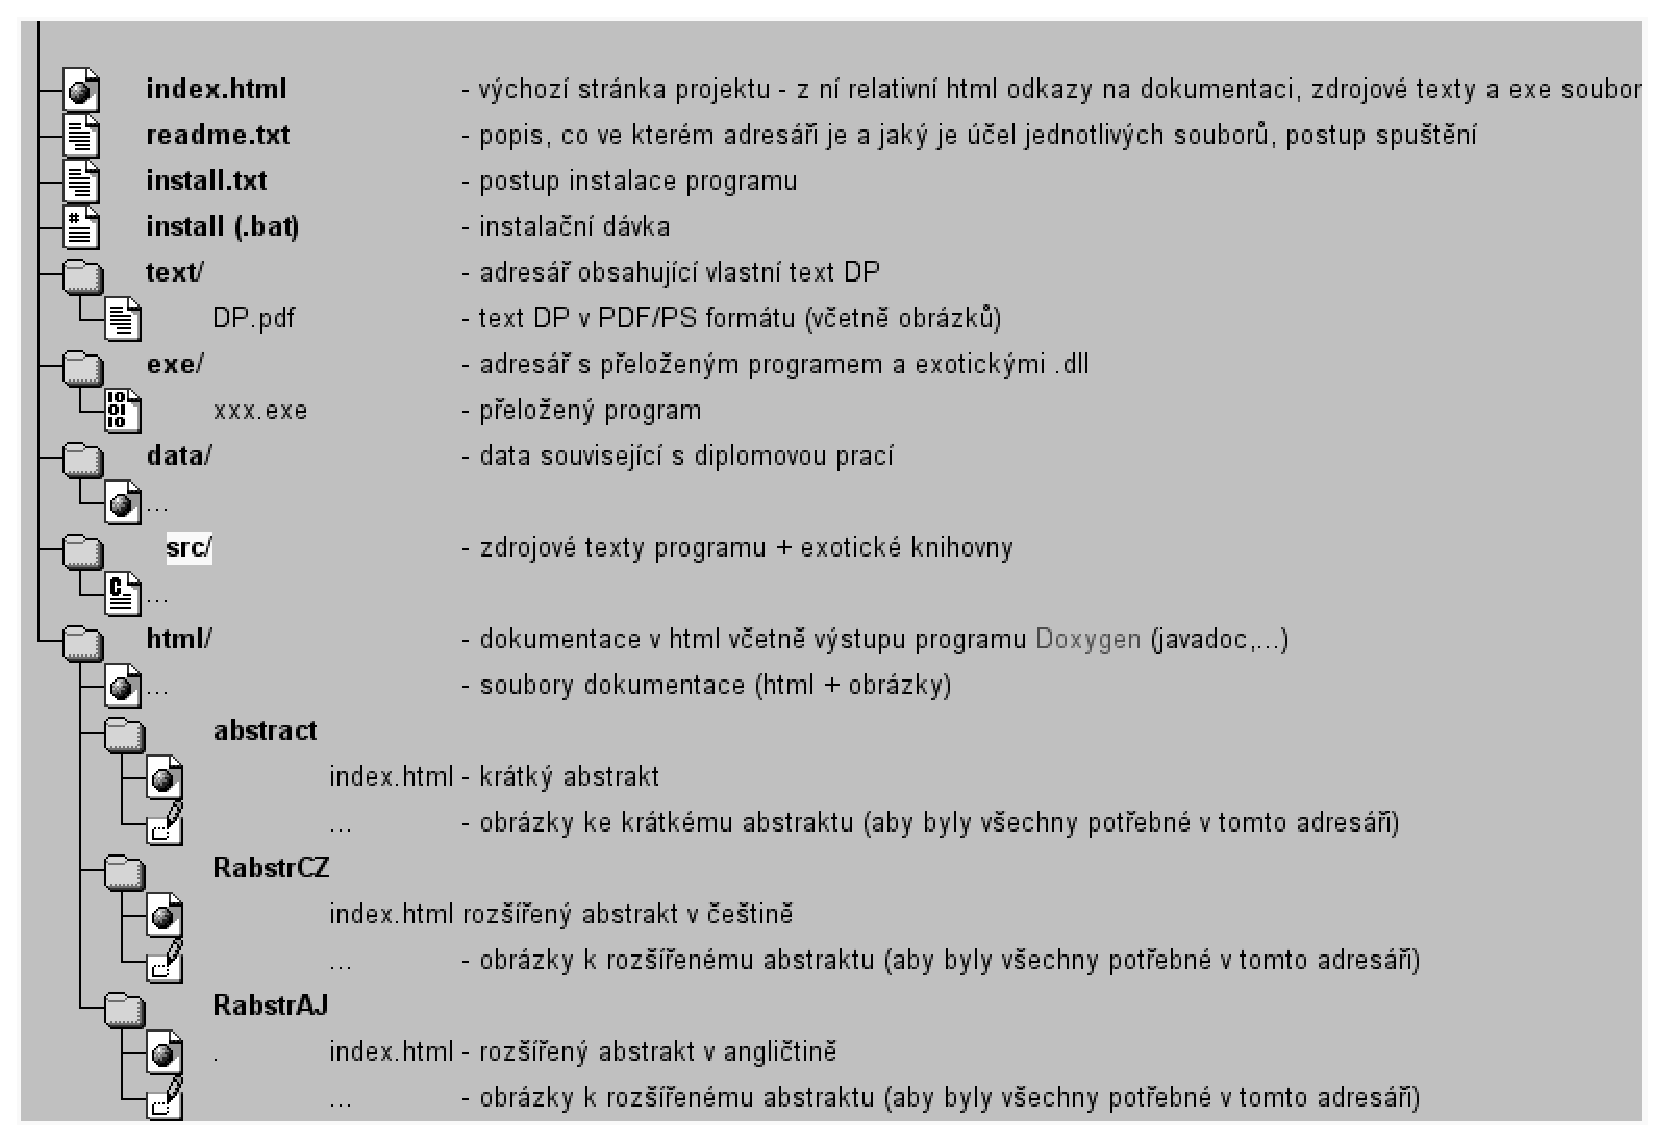
\includegraphics[width=14cm]{figures/seznamcd}
\caption{Seznam přiloženého CD --- příklad}
\label{fig:seznamcd}
\end{center}
\end{figure}

Na GNU/Linuxu si strukturu přiloženého CD můžete snadno vyrobit příkazem:\\ 
\verb|$ tree . >tree.txt|\\
Ve vzniklém souboru pak stačí pouze doplnit komentáře.

Z \textbf{README.TXT} (případne index.html apod.)  musí být rovněž zřejmé, jak programy instalovat, spouštět a jaké požadavky mají tyto programy na hardware.

Adresář \textbf{text}  musí obsahovat soubor s vlastním textem práce v PDF nebo PS formátu, který bude později použit pro prezentaci diplomové práce na WWW.

\end{document}
